\lstinputlisting[language=bash,basicstyle=\small]{python_codes/fieldstone_89/keywords}

\begin{center}
Code at \url{https://github.com/cedrict/fieldstone/tree/master/python_codes/fieldstone_89}
\end{center}

\par\noindent\rule{\textwidth}{0.4pt}

{\sl This stone was developed in collaboration wth Taco Broerse}. \index{contributors}{T. Broerse}

\par\noindent\rule{\textwidth}{0.4pt}

%%%%%%%%%%%%%%%%%%%%%%%%%%%%%%%%%%%%%%%%%%%%%%%%%%%%%%%%%%%%%%%%%%%%%%%%%%%%%%%%%%%%%%%%

What follows (and more particularly the concrete examples of deformations) 
is borrowed from the excellent site \url{https://www.continuummechanics.org/}.

%\begin{multicols}{2}

Let us start by defining the deformed vector $\vec{x}$ and the reference vector $\vec{X}$.
We assume that deformation occurs and that it transforms $\vec{X}$ into $\vec{x}$.

\paragraph{Rigid body displacement} For instance:  
\begin{eqnarray}
x &=& X + 3 \\
y &=& Y + 2 
\end{eqnarray}


\begin{center}
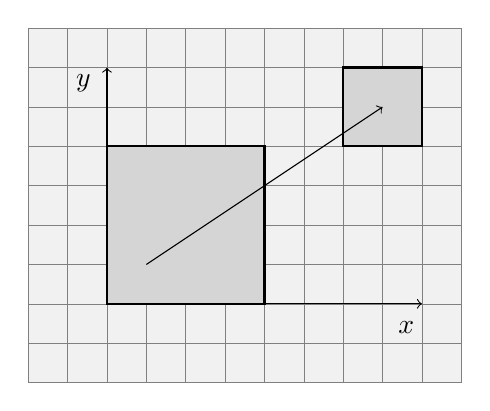
\begin{tikzpicture}
\draw[fill=gray!11,gray!11](0,0) rectangle (5.5,4.5);
\draw[step=0.5cm,gray,very thin] (0,0) grid (5.5,4.5); %background grid
\draw[fill=gray!33,thick] (1,1) -- (3,1) -- (3,3) -- (1,3) -- cycle;
\draw[thin,->]   (1,1) -- (5,1) ;
\draw[thin,->]   (1,1) -- (1,4) ;
\draw[fill=gray!33,thick] (4,3) -- (5,3) -- (5,4) -- (4,4) -- cycle; 
\node[] at (4.8,0.7) {$x$};
\node[] at (0.7,3.8) {$y$};
\draw[thin,->]   (1.5,1.5) -- (4.5,3.5) ;
\end{tikzpicture}
\end{center}



There is no deformation to speak of since the body remains the same but translated.

\paragraph{Rigid body rotation} For instance:
\begin{eqnarray}
x &=& X \cos \theta - Y \sin \theta \\ 
y &=& X \sin \theta + Y \cos \theta 
\end{eqnarray}


\begin{center}
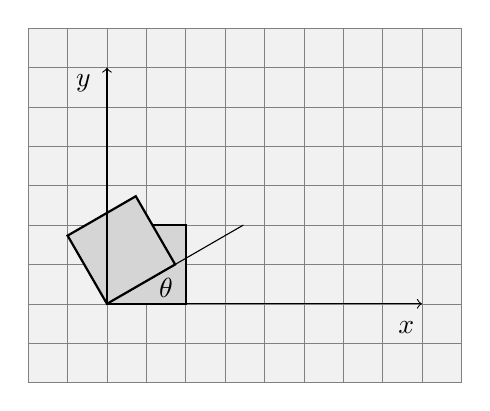
\begin{tikzpicture}
\draw[fill=gray!11,gray!11](0,0) rectangle (5.5,4.5);
\draw[step=0.5cm,gray,very thin] (0,0) grid (5.5,4.5); 
\draw[fill=gray!33,thick] (1,1) -- (2,1) -- (2,2) -- (1,2) -- cycle;
\draw[fill=gray!33,thick] (1,1) -- (1.866,1.5) -- (1.366,2.366) -- (0.5,1.866) -- cycle; 
\draw[thin,->]   (1,1) -- (5,1) ;
\draw[thin,->]   (1,1) -- (1,4) ;
\node[] at (4.8,0.7) {$x$};
\node[] at (0.7,3.8) {$y$};
\draw[thin,-] (1,1) -- (2.732,2) ;
\node[] at (1.75,1.2) {$\theta$};
\end{tikzpicture}
\end{center}



This can be rewritten as $\vec{x}={\bm F}\cdot \vec{X}$, where 
${\bm F}$ is a rotation matrix counter-clockwise about the $z$ axis (perpendicular
to the page):
\[
{\bm F} = 
\left(
\begin{array}{cc}
\cos\theta & -\sin\theta \\
\sin\theta & \cos\theta 
\end{array}
\right)
\]
Actually the body is not deformed, but simply rotated. There is no strain associated to this 
transformation. 


\paragraph{Stretching} Let us now turn to a 'real' deformation: stretching. 
For instance:
\begin{eqnarray}
x &=& 3X   \\
y &=& 2Y 
\end{eqnarray}

IMAGE

In this case the ${\bm F}$ matrix is a diagonal matrix given by 
\[
{\bm F} = 
\left(
\begin{array}{cc}
3 & 0 \\
0 & 2
\end{array}
\right)
\]
This deformation has definitely increased the area of the body by a factor 6.


\paragraph{Shearing} Another possible deformation (and a very relevant one 
in structural geology) is shearing:
\begin{eqnarray}
x &=& X   \\
y &=& \frac12 X + Y 
\end{eqnarray}
or, 
\begin{equation}
{\bm F} = 
\left(
\begin{array}{cc}
1 & 0 \\
\frac12 & 1
\end{array}
\right)
\label{eq:shearing1}
\end{equation}

IMAGE

We see that the area of the body is conserved but not its shape.

Let us now consider this shearing:
\begin{eqnarray}
x &=& X + \frac12 Y  \\
y &=& \frac12 X + Y 
\end{eqnarray}

IMAGE

Here too the shape changes and we obtain a parallelogram. AREA ?!!

So far we have then seen two types of deformation: stretching and shear, and these
can also be accompanied by rotation. 
It then makes sense to think of a deformed body as the result of successive 
shearing, stretching and rotation. 


\begin{center}
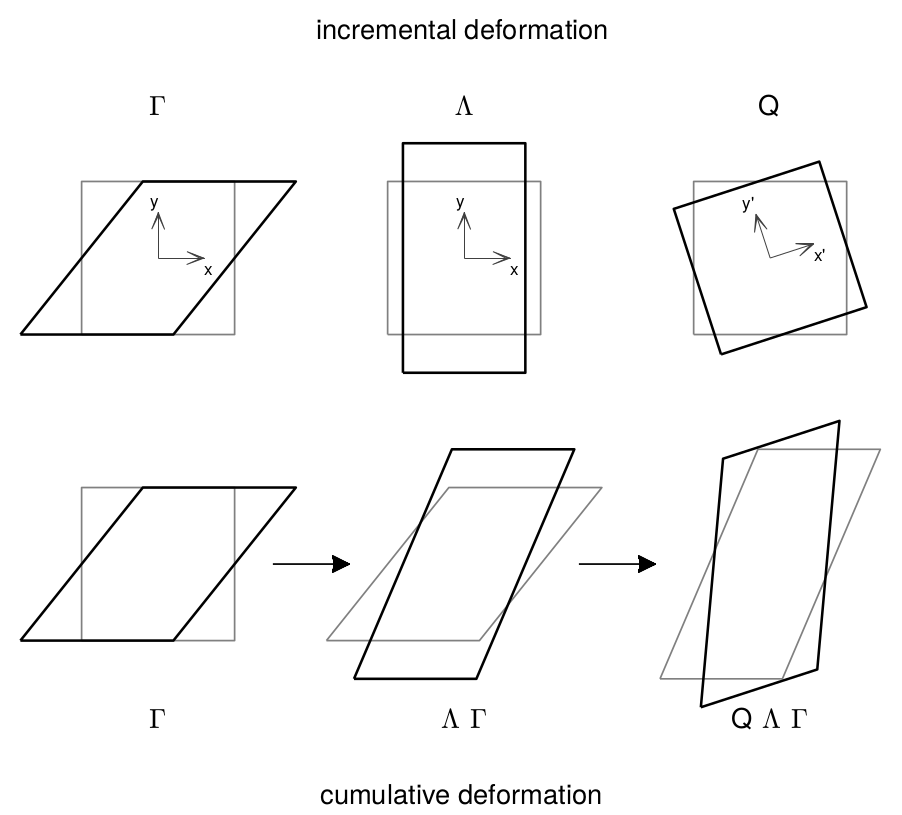
\includegraphics[width=6cm]{python_codes/fieldstone_89/images/broerse}\\
{\captionfont Taken from Broerse et al, subm.}
\end{center}


Thinking of ${\bm F}$ as the matrix which transforms $\vec{X}$ into $\vec{x}$
it then makes sense to decompose it into the product of three matrices, 
one accounting for rotation ${\bm R}$, one for stretching ${\bm \Lambda}$ and
one for shearing ${\bm \Gamma}$.
However, there is a caveat in this approach: it is easy to show that 
these transformations do not necessarily commute, i.e. the order in which 
these transformations are succesively applied matters.\todo[inline]{is this true? verify!}  

We then write
\[
{\bm F} = {\bm R} \cdot {\bm \Lambda} \cdot {\bm \Gamma}
\] 
This is called a polar decomposition:
a polar decomposition separates ${\bm F}$ into a rotation (or reflection) and a scaling of 
the space along a set of orthogonal axes\footnote{\url{https://en.wikipedia.org/wiki/Polar_decomposition}}. 
\index{general}{Polar Decomposition}

For instance, let us now consider the following transformation:
\begin{eqnarray}
x &=& 1.3X-0.375Y\\ 
y &=& 0.75X+0.65 Y
\end{eqnarray}
or, 
\[
{\bm F} = 
\left(
\begin{array}{cc}
1.3 & -0.375 \\
0.75 & 0.650
\end{array}
\right)
\]
It can be decomposed as 
\[
{\bm F} = {\bm R} \cdot {\bm U}
=
\left(
\begin{array}{cc}
0.866 & -0.5 \\
0.5 & 0.866
\end{array}
\right)
\cdot
\left(
\begin{array}{cc}
1.5 & 0 \\
0 & 0.75
\end{array}
\right)
\]
where ${\bm U}$ is the right stretch tensor, or as 
\[
{\bm F} = {\bm V} \cdot {\bm R}
=
\left(
\begin{array}{cc}
1.313 & 0.325 \\
0.325 & 0.938 
\end{array}
\right)
\cdot
\left(
\begin{array}{cc}
0.866 & -0.5 \\
0.5 & 0.866
\end{array}
\right)
\]
where ${\bm V}$ is the left stretch tensor. 
We see that ${\bm U}\ne {\bm V}$ but it can 
easily be proven that 
\[
{\bm V} = {\bm R}\cdot{\bm U}\cdot {\bm R}^T
\]
and 
\[
{\bm U} = {\bm R}^T\cdot{\bm V}\cdot {\bm R}
\]
The actual decomposition algorithm is not trivial, 
even for $2\times2$ matrices. This is nicely documented 
online\footnote{\url{http://www.continuummechanics.org/polardecomposition.html}}.

For instance, coming back to the first shearing example of Eq.~\eqref{eq:shearing1}, 
the tensor ${\bm F}$ can be written 
\[
{\bm F}= {\bm R} \cdot {\bm U}
=
\left(
\begin{array}{cc}
\cos & -\sin \\
\sin & \cos 
\end{array}
\right)
\cdot
\left(
\begin{array}{cc}
.. 
\end{array}
\right)
\]

There remains to formally define ${\bm F}$ as the deformation gradient.
\index{general}{Deformation Gradient}
It is defined as :
\[
\boxed{
{\bm F} = (\vec\nabla_X \vec{x})^T
= 
\frac{\partial \vec{x}}{\partial \vec{X}}
=
\left(
\begin{array}{cc}
\frac{\partial x}{\partial X} & 
\frac{\partial y}{\partial X} \\ \\
\frac{\partial x}{\partial Y} & 
\frac{\partial x}{\partial Y}  
\end{array}
\right)
}
\]
The transpose is necessary and best explained through example. 
Looking at the first shearing example of Eq.~\eqref{eq:shearing1}, 
we have
\begin{eqnarray}
x &=& X   \\
y &=& \frac12 X + Y 
\end{eqnarray}
and then
\[
\left(
\begin{array}{cc}
\frac{\partial x}{\partial X} & 
\frac{\partial y}{\partial X} \\ \\
\frac{\partial x}{\partial Y} & 
\frac{\partial x}{\partial Y}  
\end{array}
\right)
=
\left(
\begin{array}{cc}
1 & \frac12 \\ 
0 & 1
\end{array}
\right)
\]
while 
\[
\left(
\begin{array}{c}
x \\ y
\end{array}
\right)
=
\underbrace{
\left(
\begin{array}{cc}
1 & 0 \\
\frac12 & 1
\end{array}
\right)
}_{\bm F}
\cdot
\left(
\begin{array}{c}
X \\ Y
\end{array}
\right)
\]





We can write the displacement $\vec{u}$ as the difference between current and reference coordinates:
\[
\vec{u} = \vec{x}-\vec{X}
\]
and the deformation gradient can be reformulated as a function of the displacements:
\[
{\bm F} 
= \frac{\partial \vec{x}}{\partial \vec{X}} 
= \frac{\partial }{\partial \vec{X}} (\vec{X}+\vec{u})
= {\bm I} + \frac{\partial \vec{u}}{\partial \vec{X}} 
= {\bm I} + \vec{\nabla}\vec{u} 
\]
From this it follows that the infinitesimal strain tensor can be written
\[
\boxed{
{\bm \varepsilon} = \frac{1}{2}( \vec\nabla\vec{u} + \vec\nabla\vec{u}^T )
= \frac{1}{2} (  {\bm F} +  {\bm F}^T) - {\bm I} 
}
\]
and the rotation tensor is then 
\[
{\bm \omega} 
=\frac{1}{2}( \vec\nabla\vec{u} - \vec\nabla\vec{u}^T )
= \frac{1}{2} (  {\bm F} -  {\bm F}^T)
\]






%\end{multicols}

\newpage
This stone has two purposes:
\begin{itemize}
\item put the theory above into practice 
\item show that the 'standard' way of integrating strain on Lagrangian markers in 
geodynamical codes is merely an approximation and that this approximation 
no longer holds for large deformations/rotations. In other words, 
integrated strain rates lose their physical meaning when 
the deformation becomes large!
\end{itemize}


\note{
The deformation gradient tensor ${\bm F}$ is computed in the middle of
each cell at a given time $t$ as follows:
\[
{\bm F}(t)
=
\left(
\begin{array}{cc}
F_{xx} & F_{xy} \\
F_{yx} & F_{yy} 
\end{array}
\right)
=
{\bm I}+
\left(
\begin{array}{cc}
\frac{\partial (x(t)-x_0)}{\partial x}  & \frac{\partial (x(t)-x_0)}{\partial y}  \\
\frac{\partial (y(t)-y_0)}{\partial x}  & \frac{\partial (y(t)-y_0)}{\partial y}  
\end{array}
\right)
\]
In what follows we omit the time dependence '$(t)$'.
Each cell is assumed to be a $Q_1$ quadrilateral with a marker at each corner. We therefore store the 
initial position of markers, and make use of bilinear $Q_1$ shape functions to compute the derivatives
above in the center of the cell.

\begin{enumerate}
\item The right Cauchy-Green deformation tensor is defined as
\[
{\bm C} = {\bm F}^T {\bm F}
\]
\item 
We then find the eigenvalues of ${\bm C}$:
\[
\mu_{1,2} = \frac{1}{2}(C_{xx}+C_{yy}) \pm \sqrt{ \frac{1}{4}(C_{xx}-C_{yy})^2 + C_{xy}^2   }
\]
\item We compute the two invariants:
\[
I_C = \mu_1+\mu_2 \qquad II_C = \mu_1\mu_2 
\]
\item Compute invariants of right stretch tensor U
\[
I_U=\sqrt{I_C+2\sqrt{II_C}}
\qquad
II_U=\sqrt{II_C}
\]
\item compute right stretch tensor ${\bm U}$
\[
{\bm U} = \frac{{\bm C}+ II_U {\bm I}}{I_U}
\]
\item compute inverse of ${\bm U}$
\[
{\bm U}^{-1} = - I_U \frac{{\bm C}- (II_U+I_C){\bm I}}{II_U(II_U+I_C)+II_C}
\]
\item compute rotation matrix ${\bm R}={\bm F}{\bm U}^{-1}$

\item compute left stretch tensor ${\bm V}={\bm F}{\bm R}^T$

\item Compute eigenvalues of ${\bm V}$, which are the square roots of those of ${\bm C}$
\[
\lambda_1 = \sqrt{\mu_1}
\qquad
\lambda_2 = \sqrt{\mu_2}
\]

\end{enumerate}
}













\newpage
%%%%%%%%%%%%%%%%%%%%%%%%%%%%%%%%%%%%%%%%%%%%%%%%%%%%%%%%%%%%%%%%%%%%%%5
\subsection*{The shear band (experiment=1)}

The domain is a rectangle of size $L_x\times L_y$ discretised by nelx $\times$ nely $Q_2$ elements.
The following velocity field is precribed in the domain:
\begin{eqnarray}
u(x,y)&=&0 \\
v(x,y)&=&\text{erf} [A(x-L_x/2)]
\end{eqnarray}

A swarm of $41\times41$ markers is then placed in the domain, 
and they are then painted as shown here:
\begin{center}

\includegraphics[width=5.6cm]{python_codes/fieldstone_89/results/shearband/init/grid}
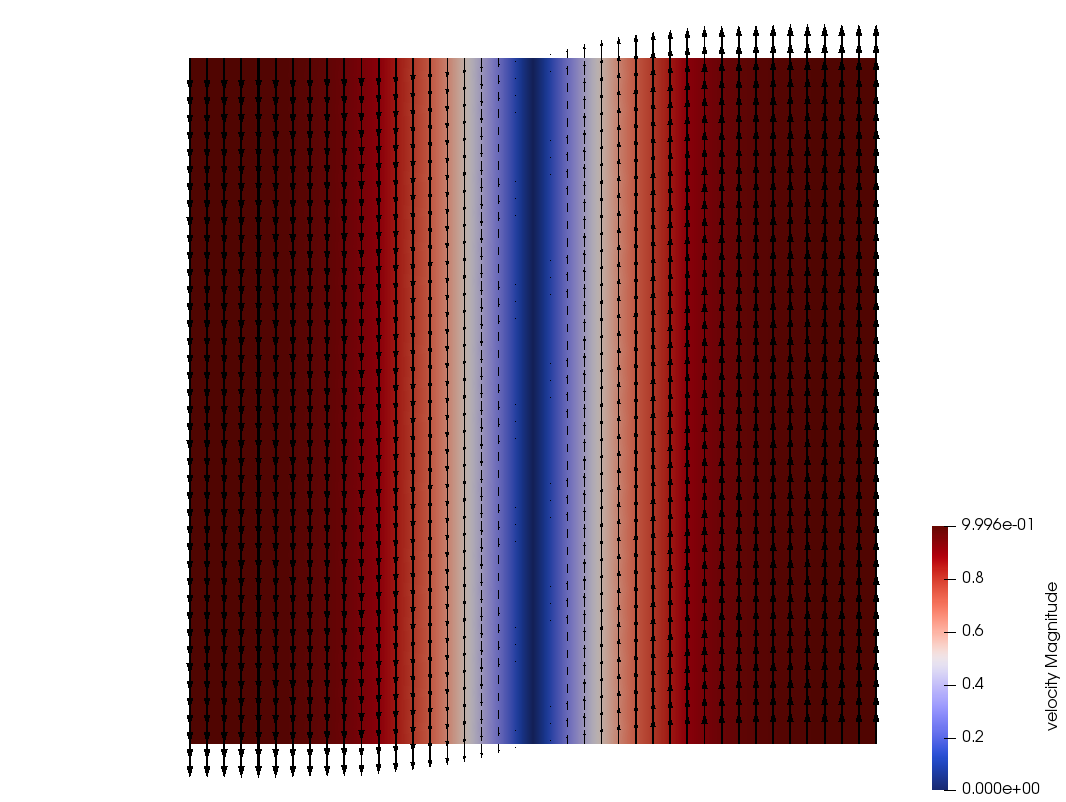
\includegraphics[width=5.6cm]{python_codes/fieldstone_89/results/shearband/init/vel}
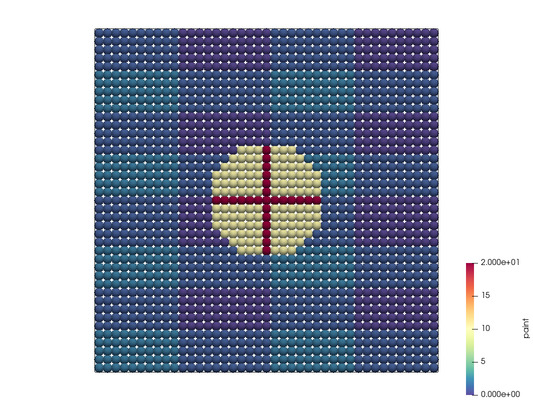
\includegraphics[width=5.6cm]{python_codes/fieldstone_89/results/shearband/init/markers}\\
{\captionfont Domain is unit square, resolution $20\times20$ elements. $A=5$. 
Left: Eulerian grid; Middle: velocity field; Right: marker initial position.}
\end{center}

A time loop is implemented. At each time step the velocity field of the grid is 
interpolated onto each marker that is in turn advected with a simple euler step. 
\[
\vec{x}(t+\delta t) = \vec{x}(t) + \vec\upnu \; \delta t
\]
Note that the timestep value $\delta t$ is controlled by means of a CFL condition 
with ${\cal C}=0.1$. Likewise, the components of the strain rate tensor are computed on each marker and 
used to update the strain on each marker:
\[
\varepsilon_{ij}(t+\delta t) = \varepsilon_{ij}(t) + \dot\varepsilon_{ij}(t) \; \delta t
\]
These markers form a Lagrangian mesh which deforms over time:
\begin{center}
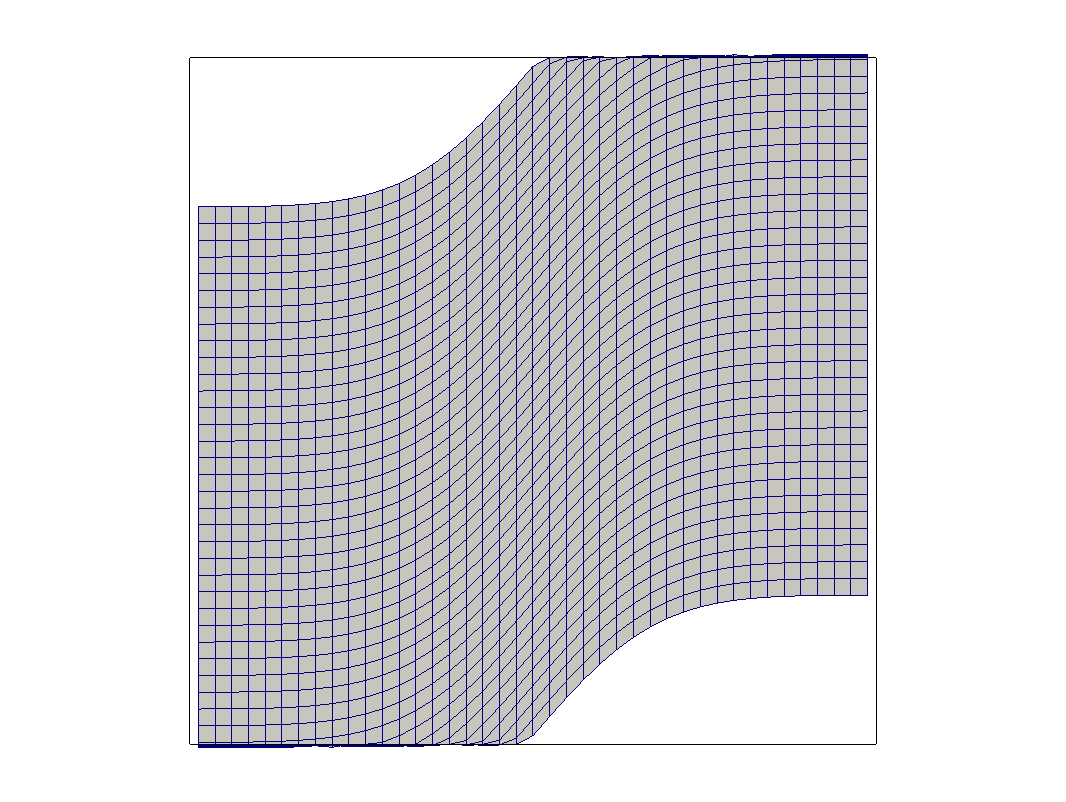
\includegraphics[width=6cm]{python_codes/fieldstone_89/results/shearband/init/swarm_mesh}
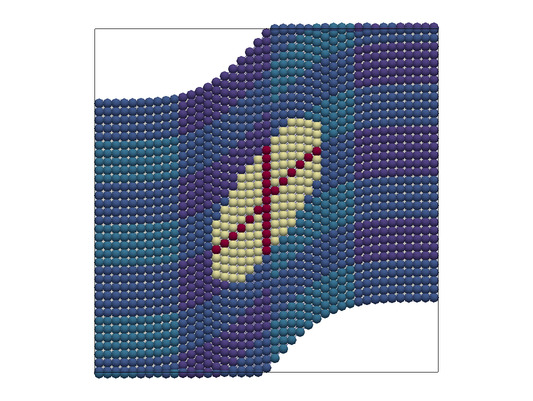
\includegraphics[width=6cm]{python_codes/fieldstone_89/results/shearband/init/swarm_paint}\\
{\captionfont Lagrangian mesh after 50 time steps.}
\end{center}
Markers which are advected outside of the domain are simply flagged inactive. 

At each time step the cumulative strain $\varepsilon_{ij}$ components are
computed at the center of the marker cells, as well as the principal strains $\varepsilon_1$ 
and $\varepsilon_2$ and the direction $\theta_\varepsilon$ of the principal strain:

\begin{center}
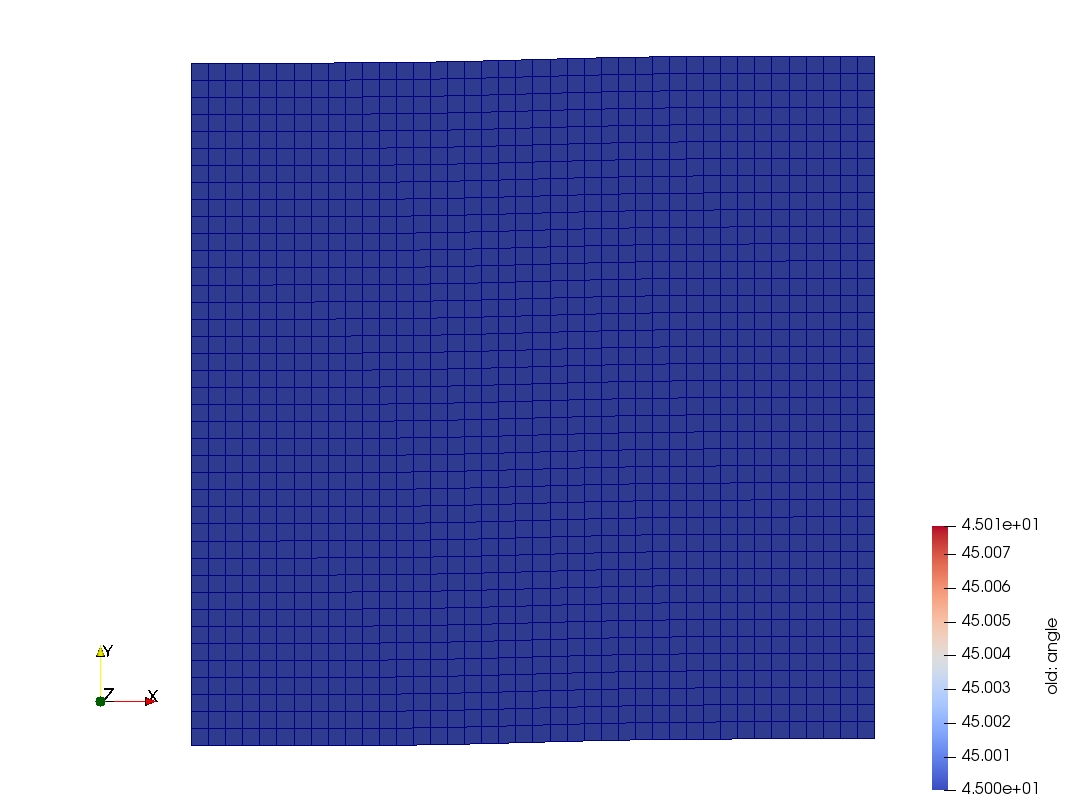
\includegraphics[width=4cm]{python_codes/fieldstone_89/results/shearband/old_angle_00}
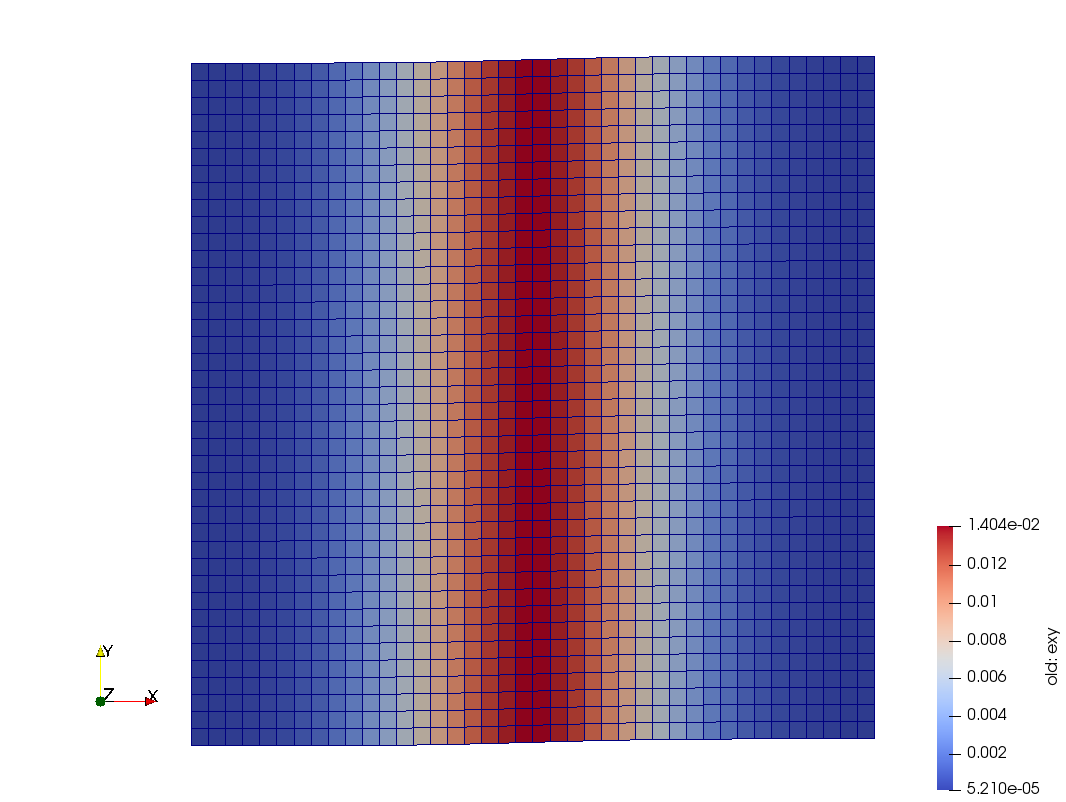
\includegraphics[width=4cm]{python_codes/fieldstone_89/results/shearband/old_exy_00}\\
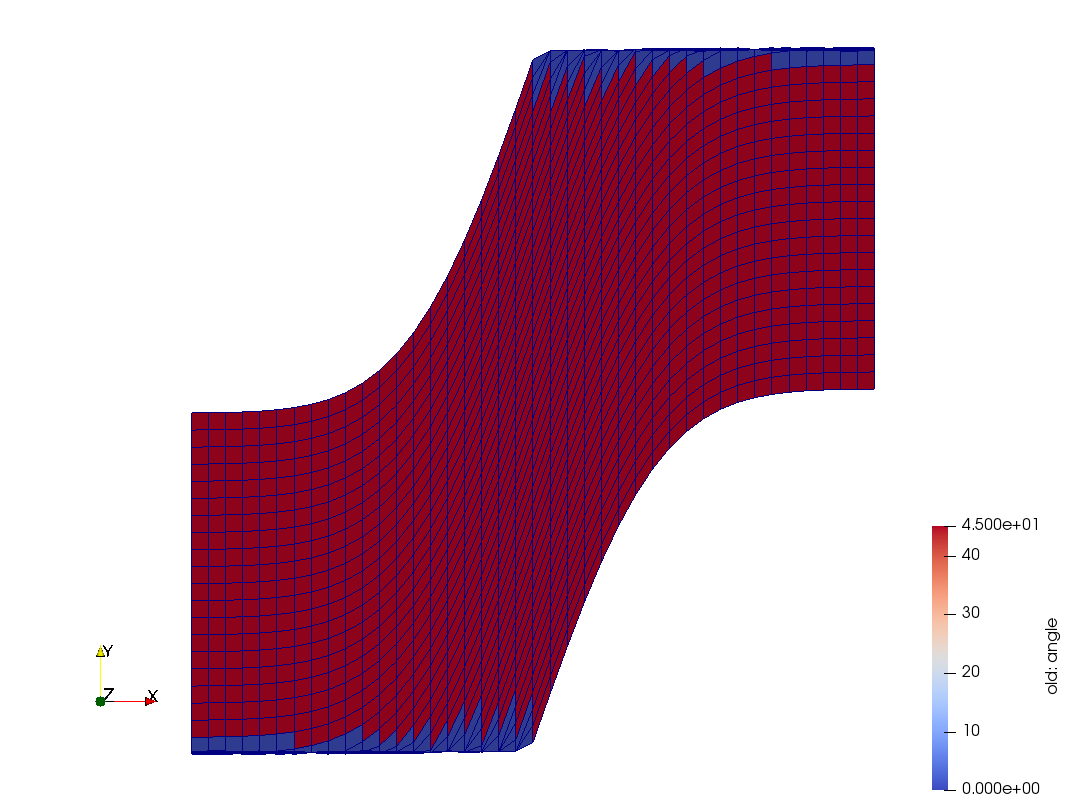
\includegraphics[width=4cm]{python_codes/fieldstone_89/results/shearband/old_angle_100}
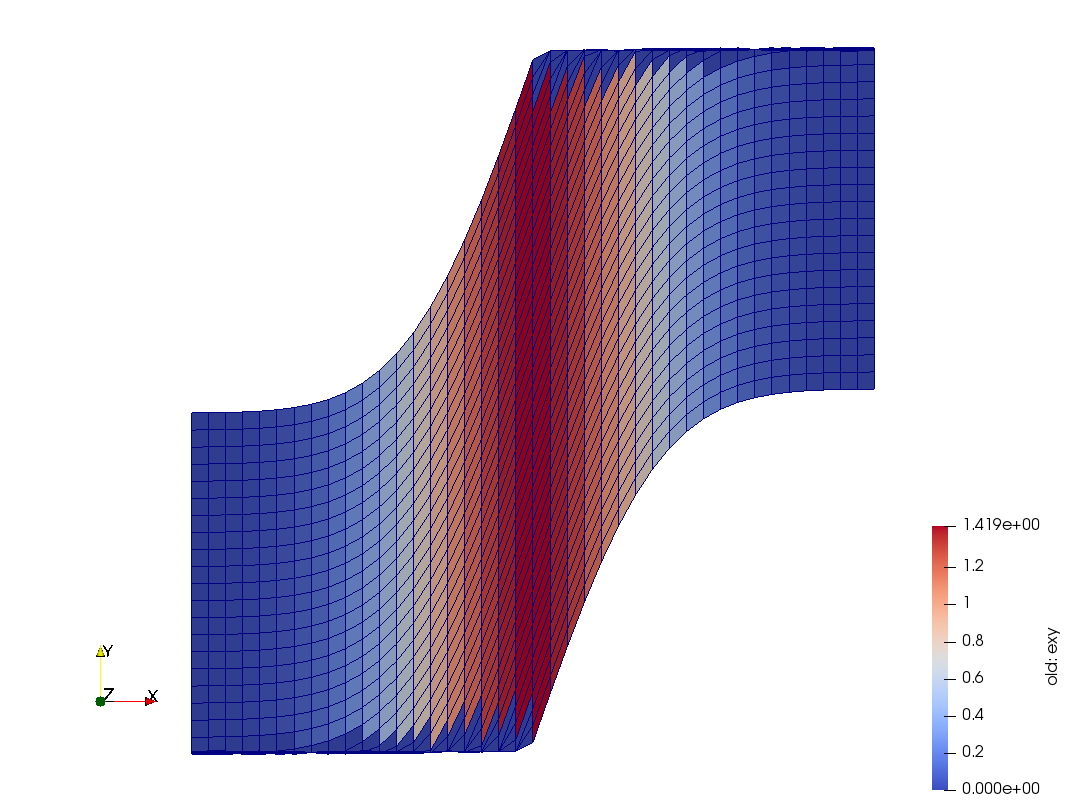
\includegraphics[width=4cm]{python_codes/fieldstone_89/results/shearband/old_exy_100}\\
{\captionfont From left to right: angle, principal strain directions, $\varepsilon_{xy}$.
Top row: first time step; Bottom row: 100th time step.}
\end{center}


\begin{center}
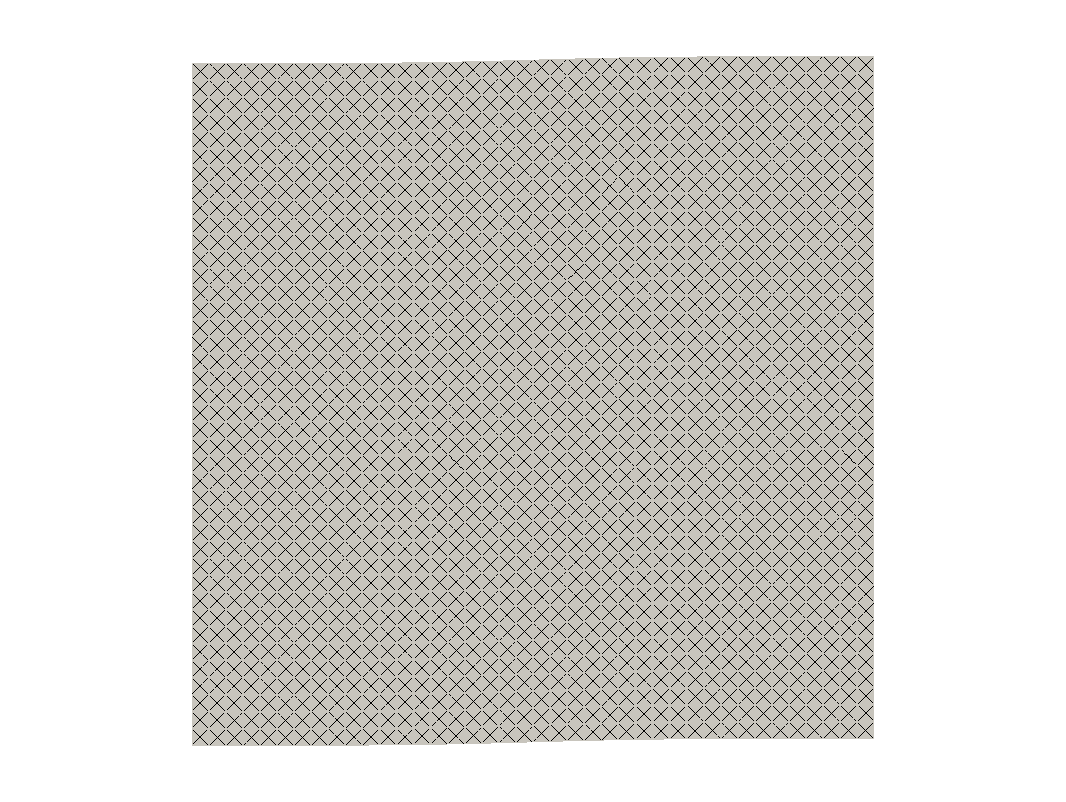
\includegraphics[width=4cm]{python_codes/fieldstone_89/results/shearband/old_dirs0000}
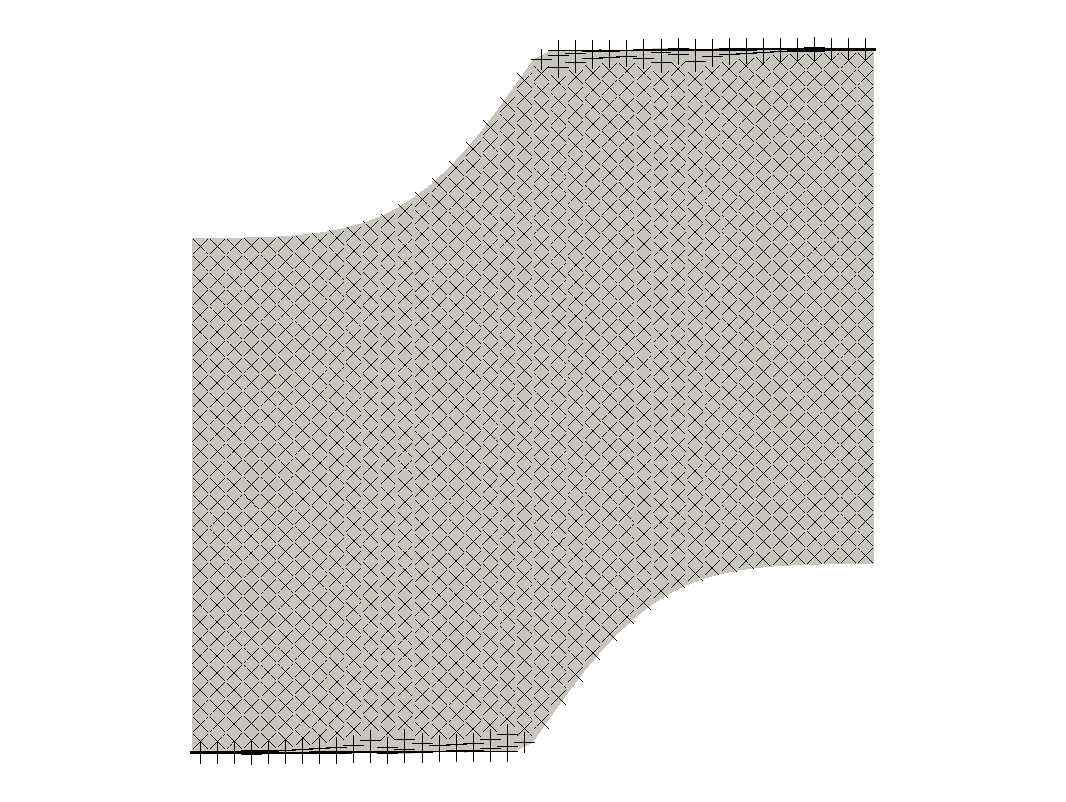
\includegraphics[width=4cm]{python_codes/fieldstone_89/results/shearband/old_dirs0005}
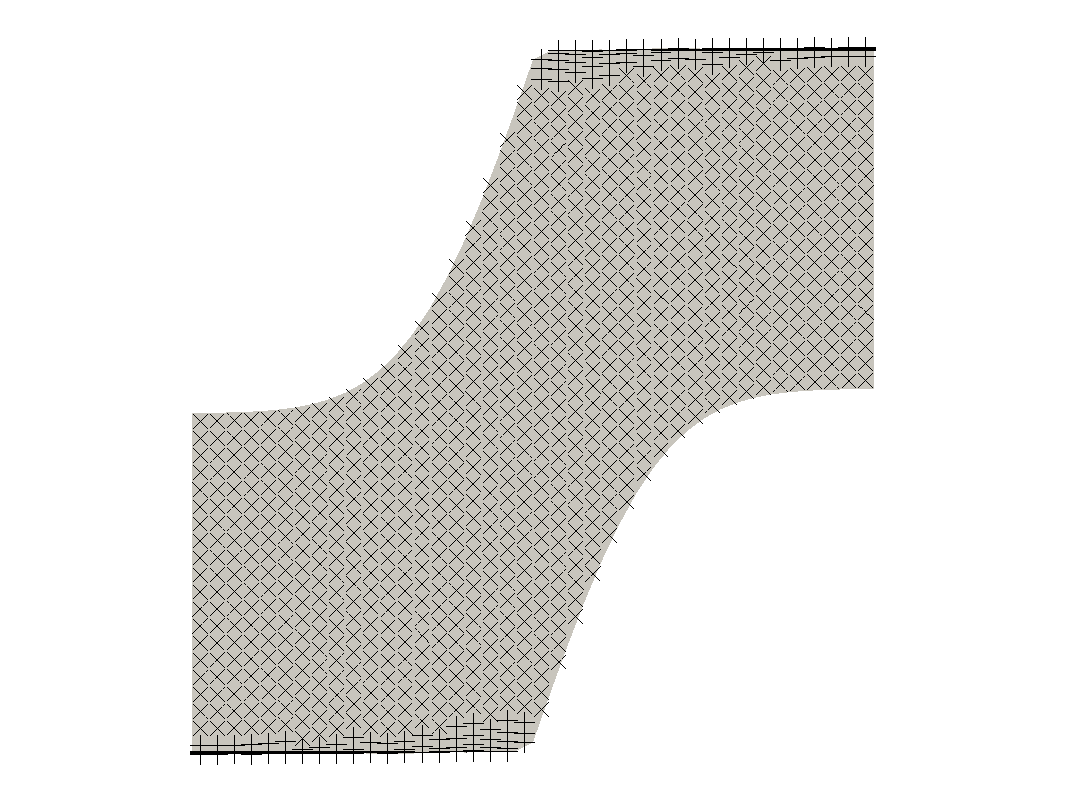
\includegraphics[width=4cm]{python_codes/fieldstone_89/results/shearband/old_dirs0010}\\
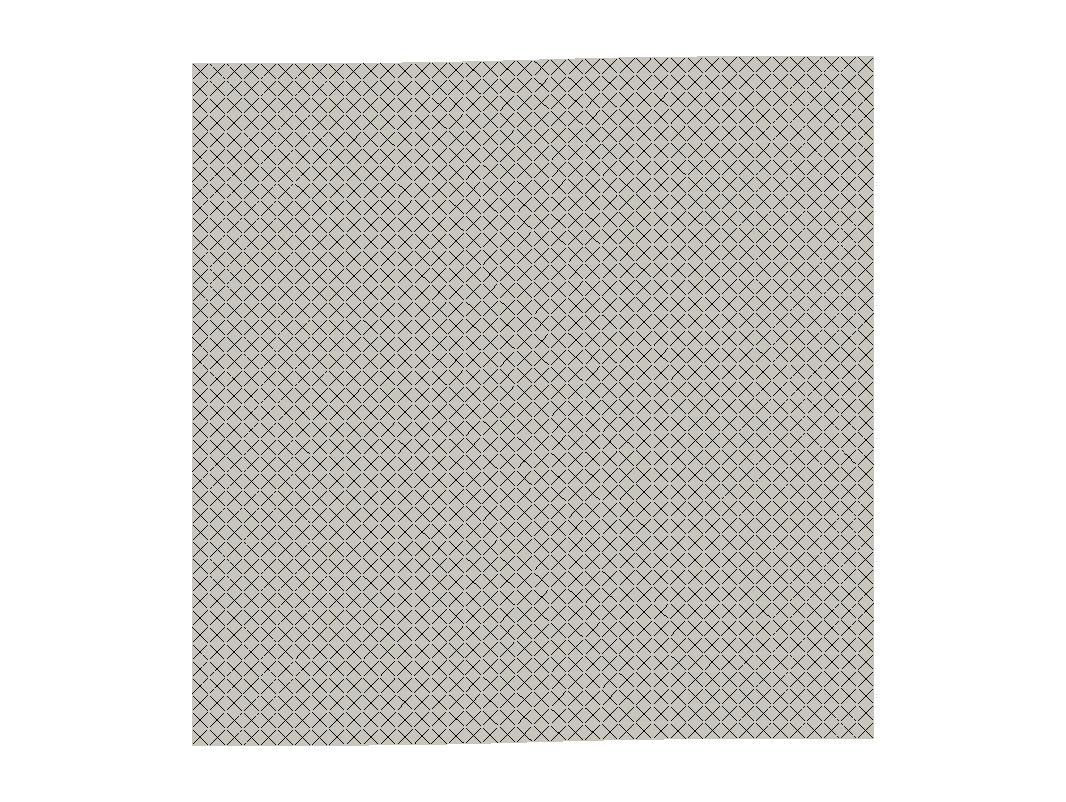
\includegraphics[width=4cm]{python_codes/fieldstone_89/results/shearband/new_dirs0000}
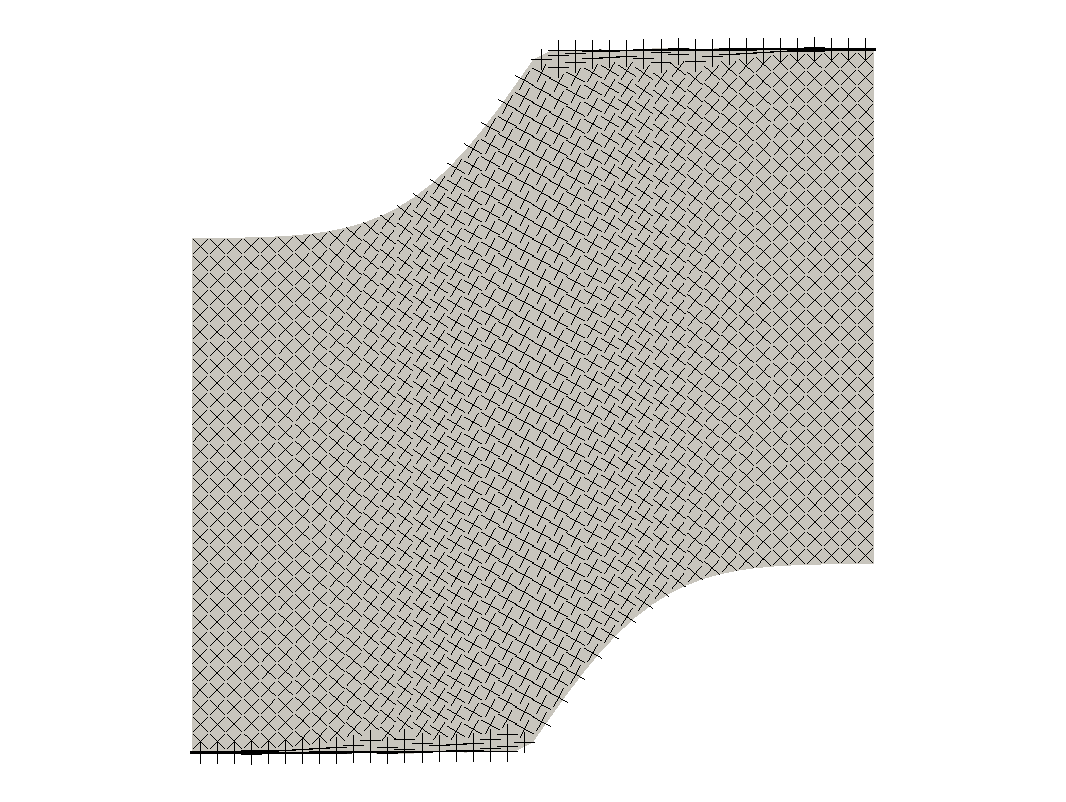
\includegraphics[width=4cm]{python_codes/fieldstone_89/results/shearband/new_dirs0005}
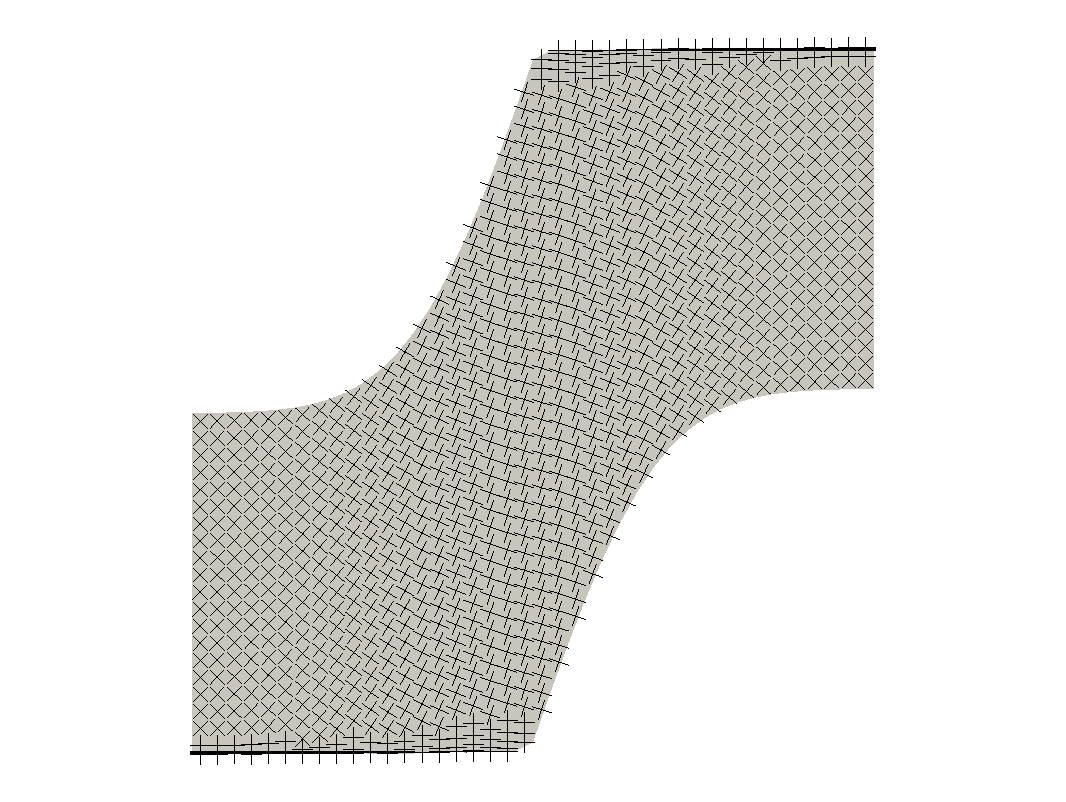
\includegraphics[width=4cm]{python_codes/fieldstone_89/results/shearband/new_dirs0010}\\
\end{center}


A single cell is chosen in the middle of the domain and its strain values 
recorded over time in a file:
\begin{center}
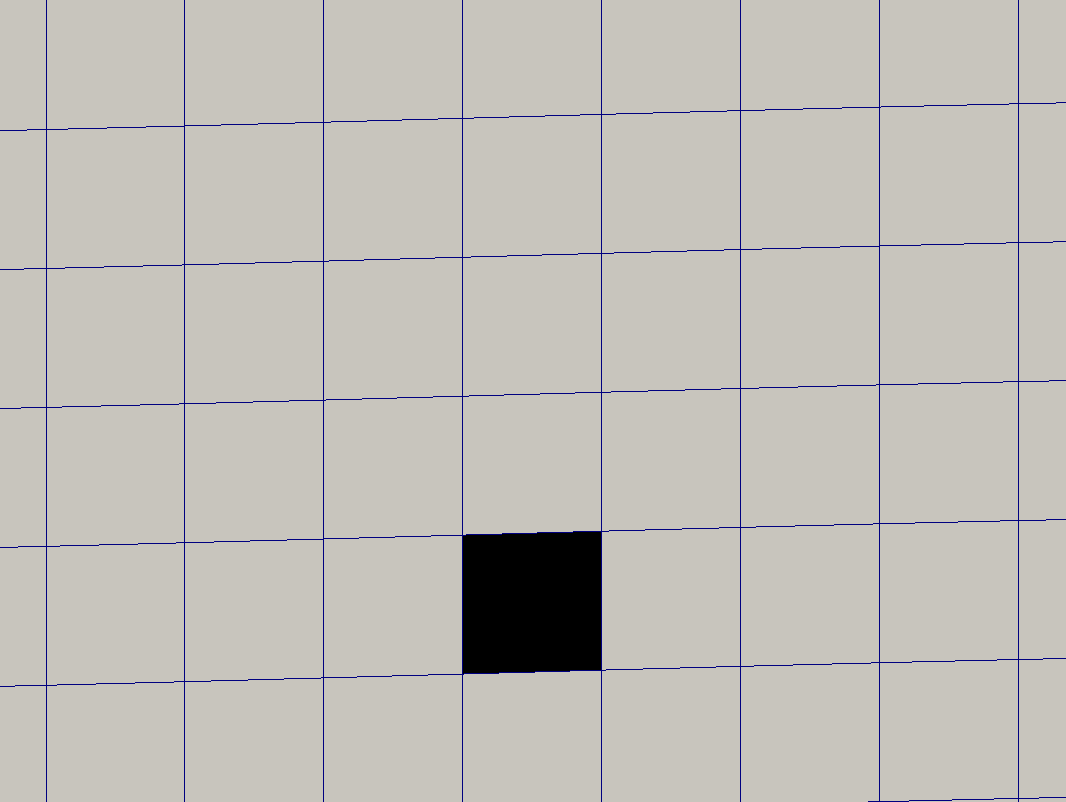
\includegraphics[width=4cm]{python_codes/fieldstone_89/results/shearband/target0000.png}
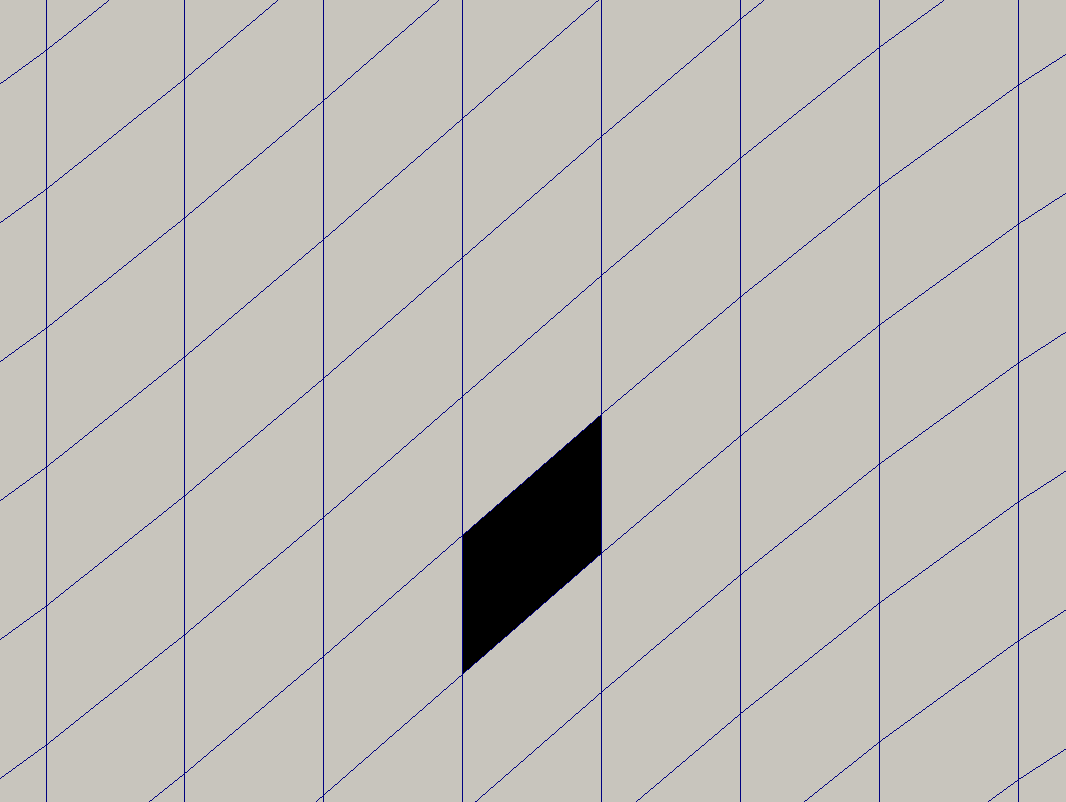
\includegraphics[width=4cm]{python_codes/fieldstone_89/results/shearband/target0003.png}
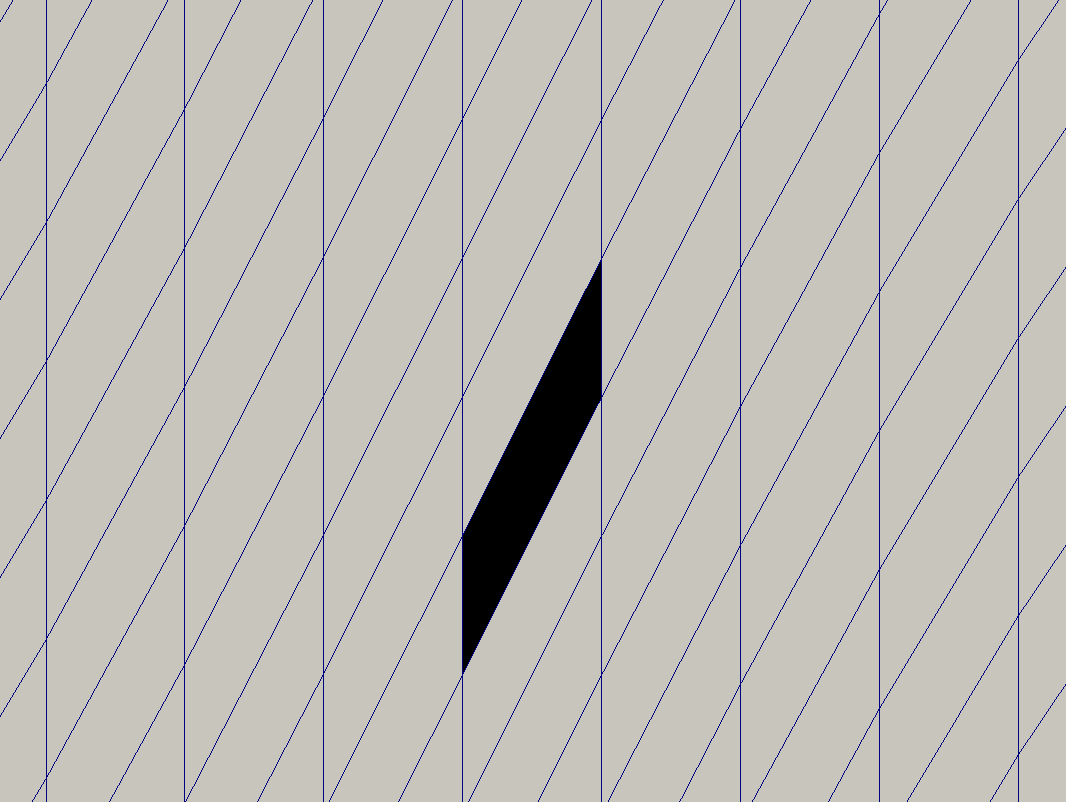
\includegraphics[width=4cm]{python_codes/fieldstone_89/results/shearband/target0007.png}
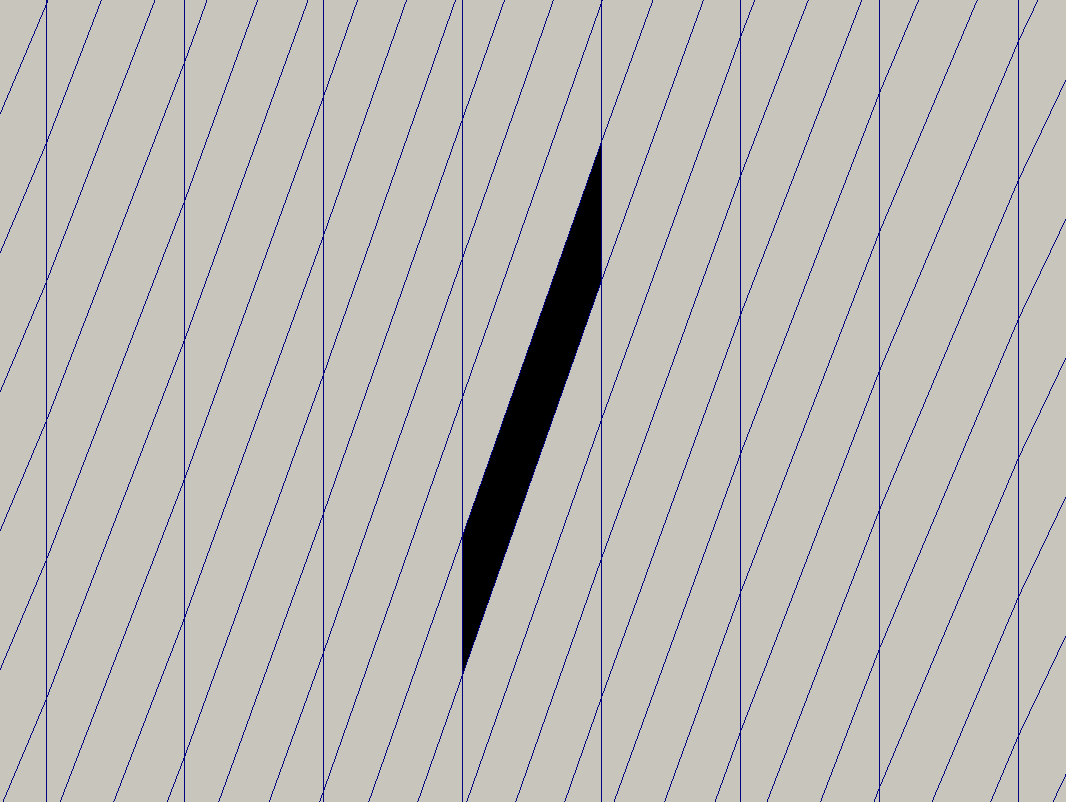
\includegraphics[width=4cm]{python_codes/fieldstone_89/results/shearband/target0010.png}\\
{\captionfont Cell undergoing deformation.}
\end{center}

\begin{center}
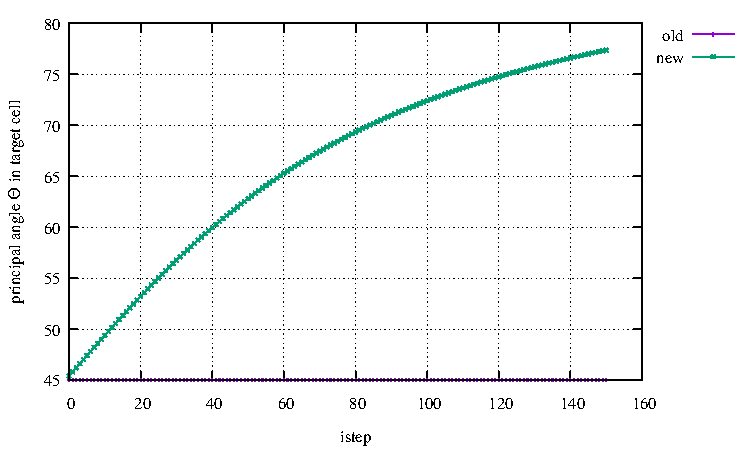
\includegraphics[width=5.5cm]{python_codes/fieldstone_89/results/shearband/principal_angle.pdf}
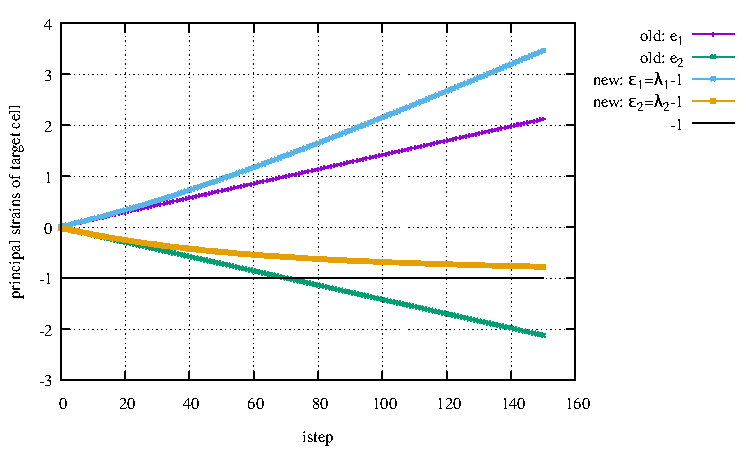
\includegraphics[width=5.5cm]{python_codes/fieldstone_89/results/shearband/principal_strains.pdf}
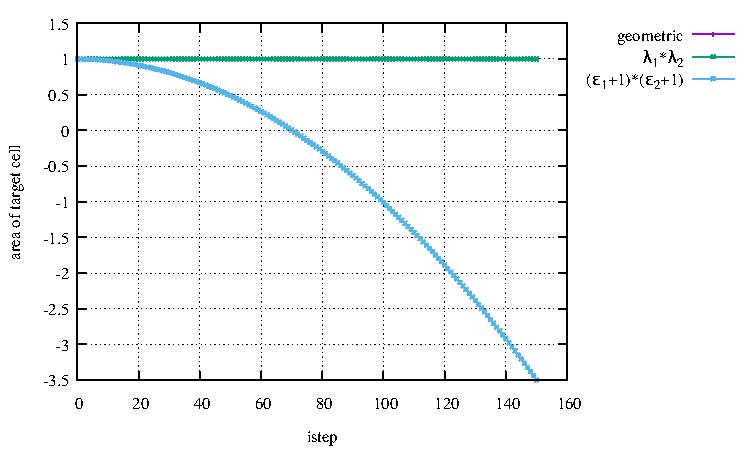
\includegraphics[width=5.5cm]{python_codes/fieldstone_89/results/shearband/area.pdf}\\
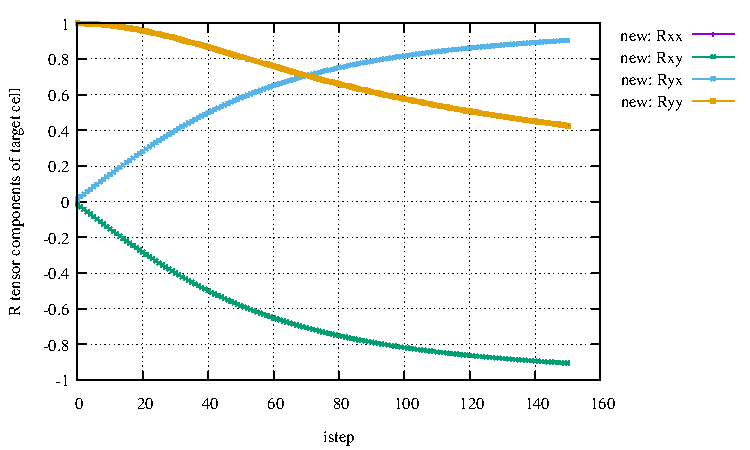
\includegraphics[width=5.5cm]{python_codes/fieldstone_89/results/shearband/R.pdf}
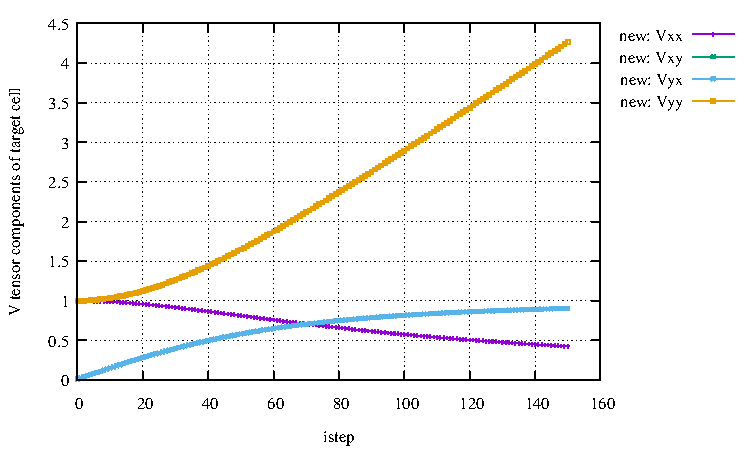
\includegraphics[width=5.5cm]{python_codes/fieldstone_89/results/shearband/V.pdf}
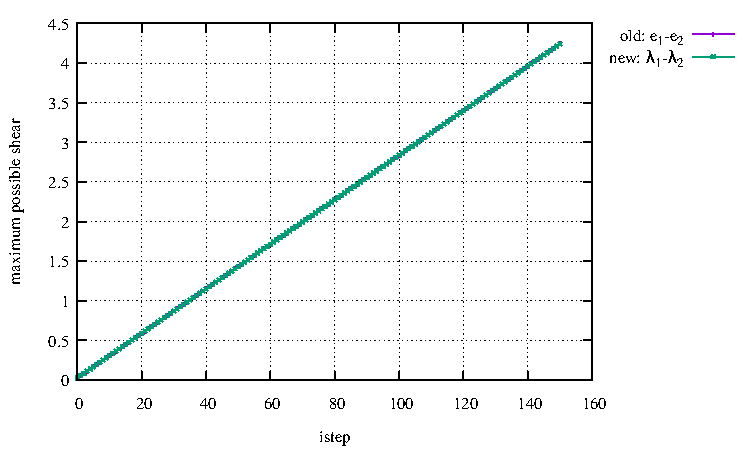
\includegraphics[width=5.5cm]{python_codes/fieldstone_89/results/shearband/maximum_shear.pdf}\\
{\captionfont Time evolution of the principal angle $\theta_\varepsilon$, 
the strain principal values and the area of the target cell.}
\end{center}










\newpage
%%%%%%%%%%%%%%%%%%%%%%%%%%%%%%%%%%%%%%%%%%%%%%%%%%%%%%%%%%%%%%%%%%%%%%5
\subsection*{The vertical extension (experiment=2)} 

\begin{eqnarray}
u(x,y)&=&0 \\
v(x,y)&=&y
\end{eqnarray}




\begin{center}
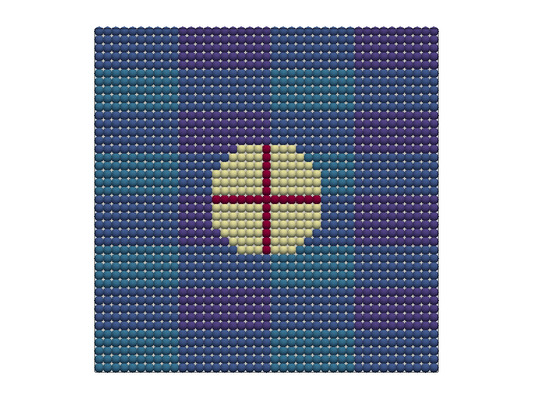
\includegraphics[width=4cm]{python_codes/fieldstone_89/results/vertical/paint0000}
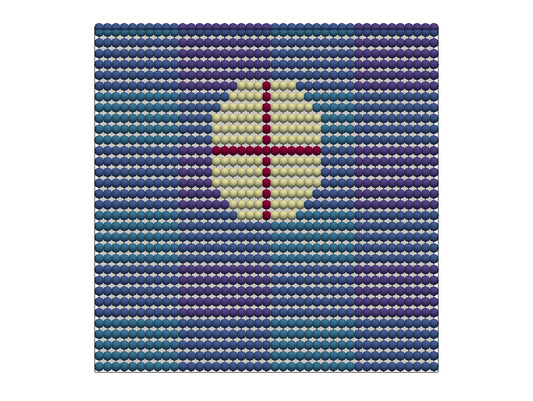
\includegraphics[width=4cm]{python_codes/fieldstone_89/results/vertical/paint0005}
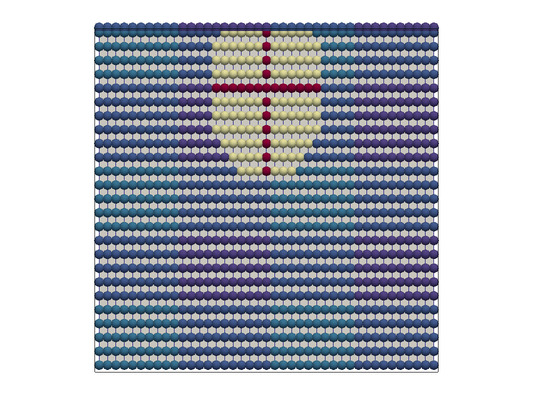
\includegraphics[width=4cm]{python_codes/fieldstone_89/results/vertical/paint0010}
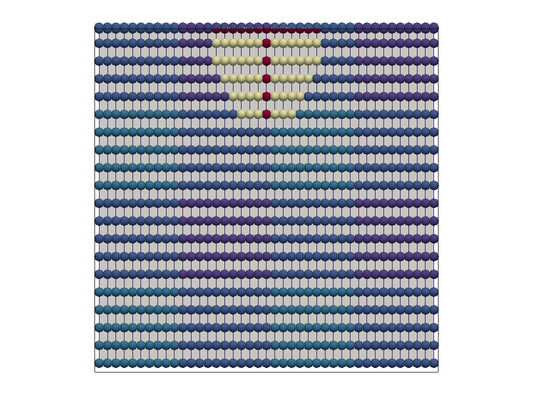
\includegraphics[width=4cm]{python_codes/fieldstone_89/results/vertical/paint0015}
\end{center}

\begin{center}
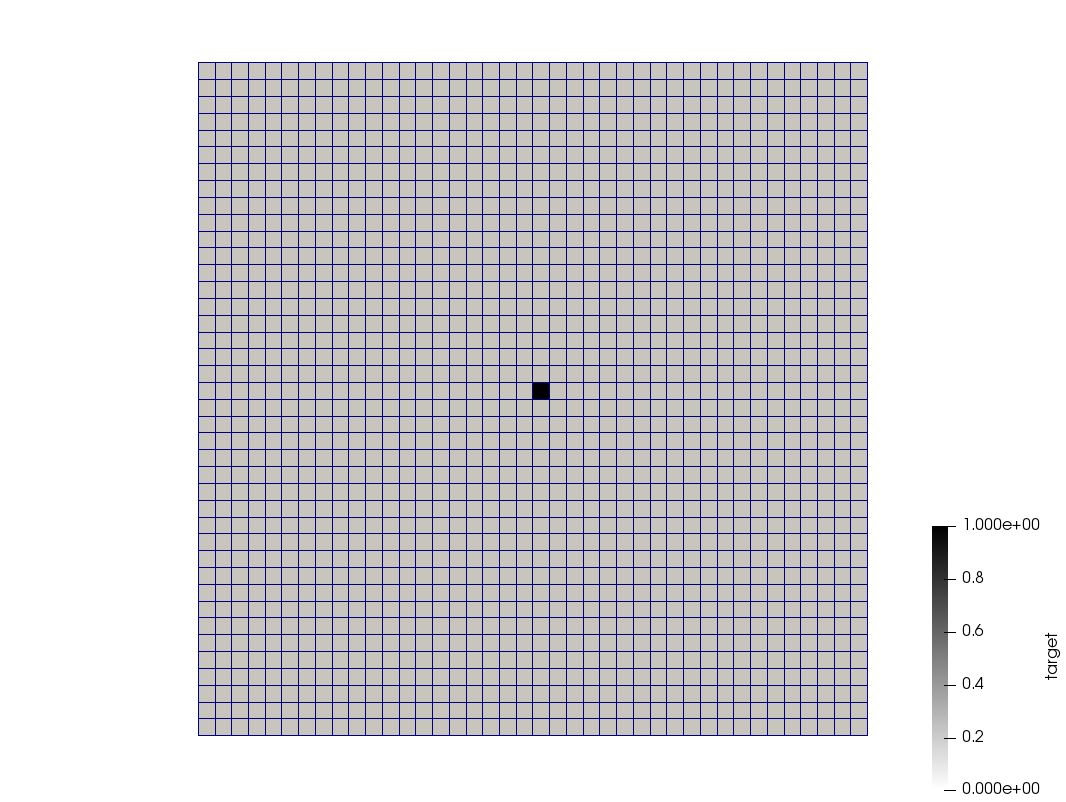
\includegraphics[width=4cm]{python_codes/fieldstone_89/results/vertical/target0000}
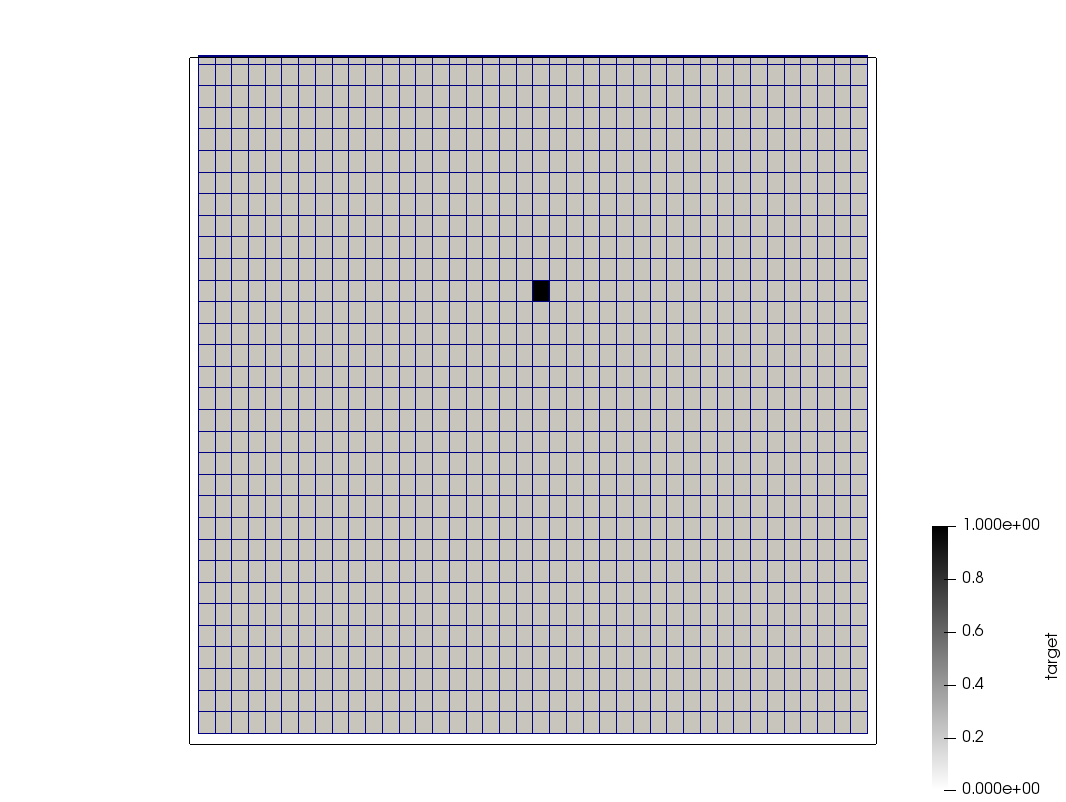
\includegraphics[width=4cm]{python_codes/fieldstone_89/results/vertical/target0005}
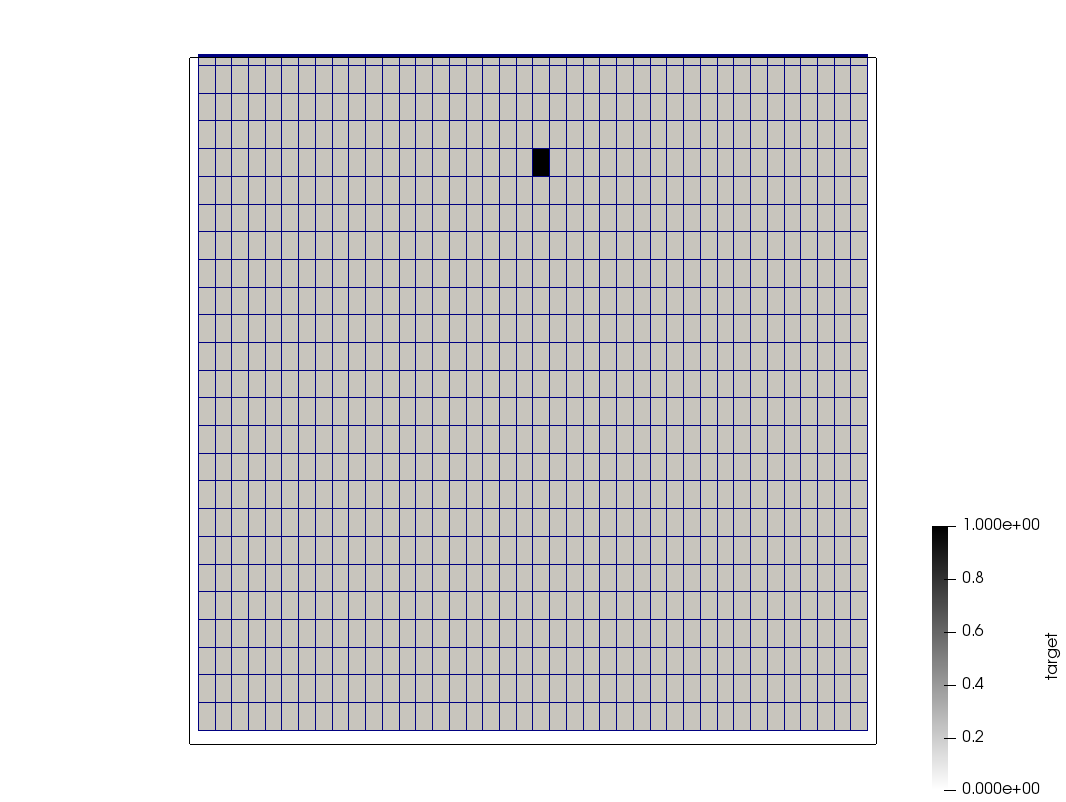
\includegraphics[width=4cm]{python_codes/fieldstone_89/results/vertical/target0010}
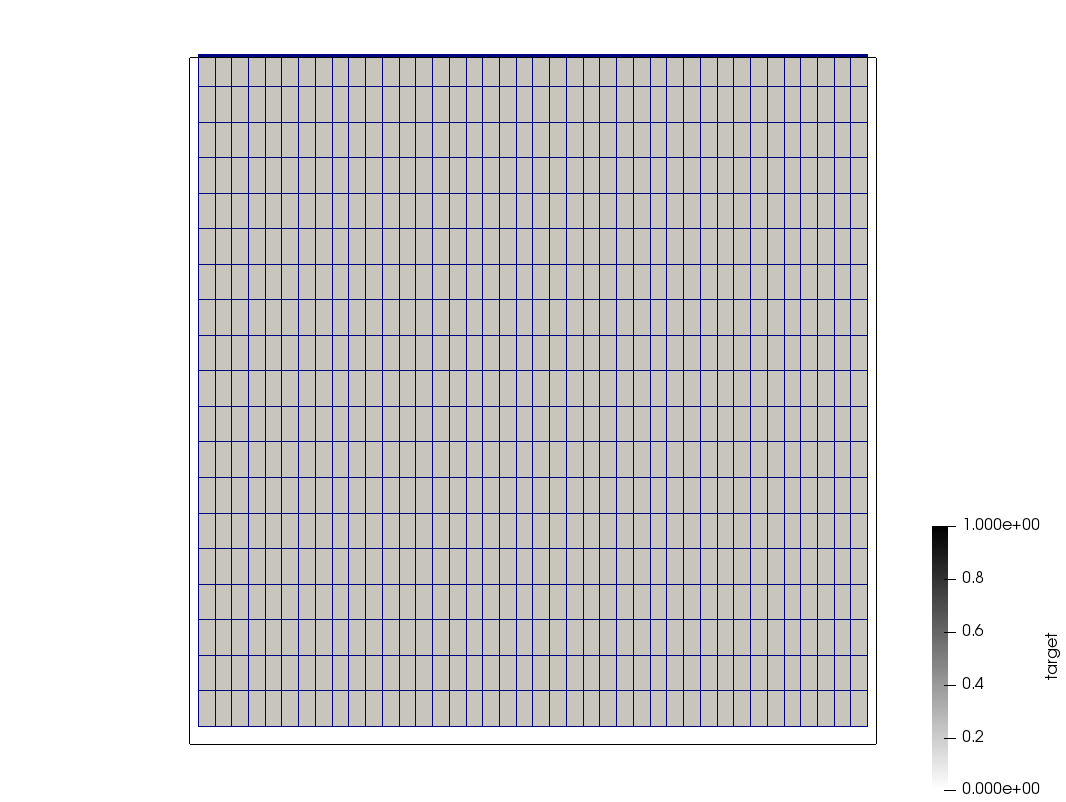
\includegraphics[width=4cm]{python_codes/fieldstone_89/results/vertical/target0015}
\end{center}

\begin{center}
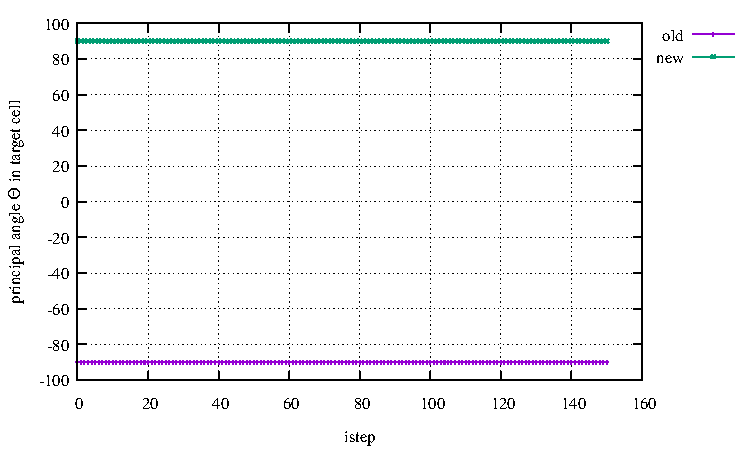
\includegraphics[width=5.5cm]{python_codes/fieldstone_89/results/vertical/principal_angle.pdf}
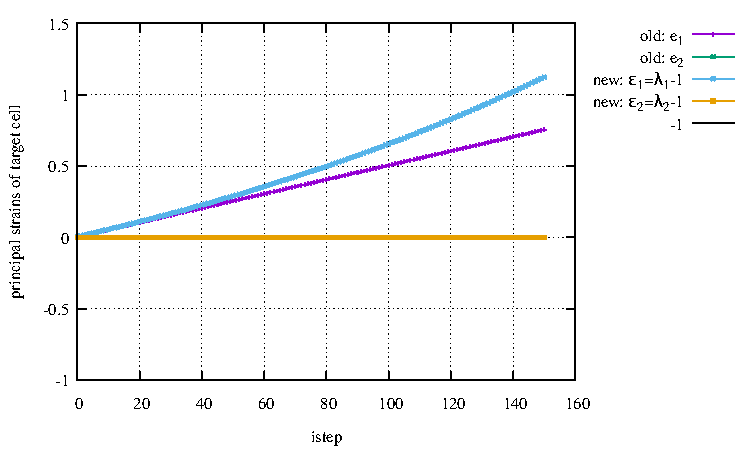
\includegraphics[width=5.5cm]{python_codes/fieldstone_89/results/vertical/principal_strains.pdf}
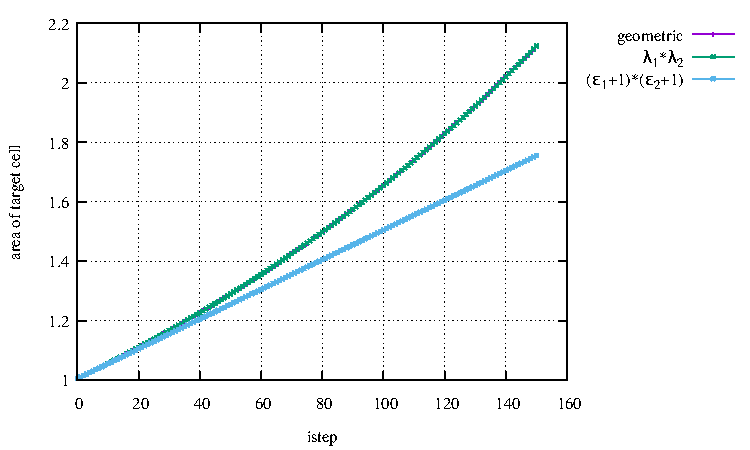
\includegraphics[width=5.5cm]{python_codes/fieldstone_89/results/vertical/area.pdf}\\
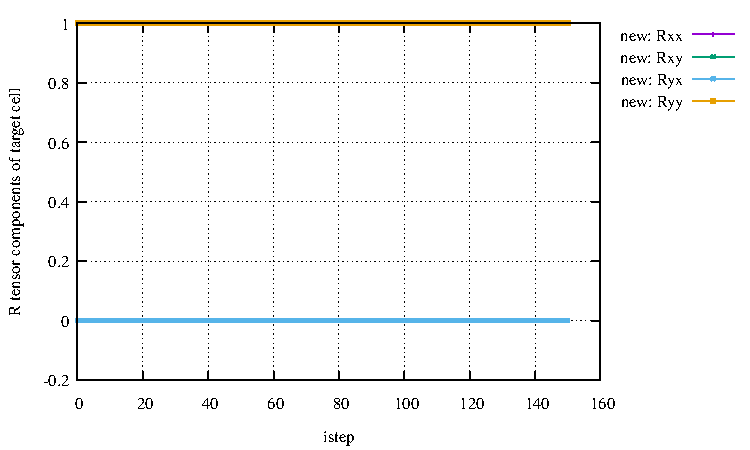
\includegraphics[width=5.5cm]{python_codes/fieldstone_89/results/vertical/R.pdf}
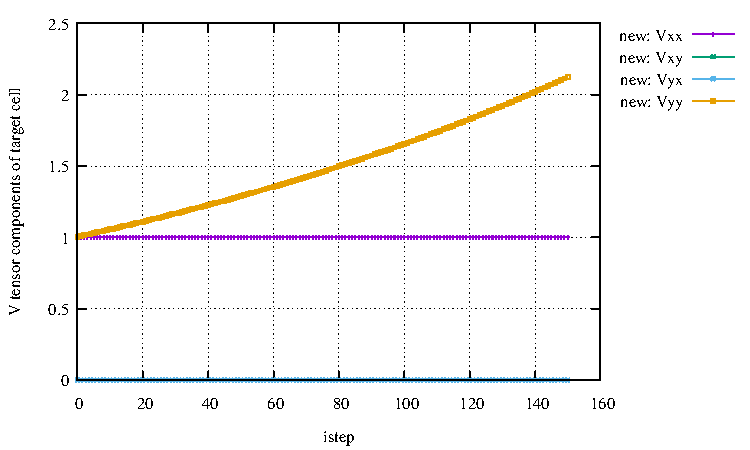
\includegraphics[width=5.5cm]{python_codes/fieldstone_89/results/vertical/V.pdf}
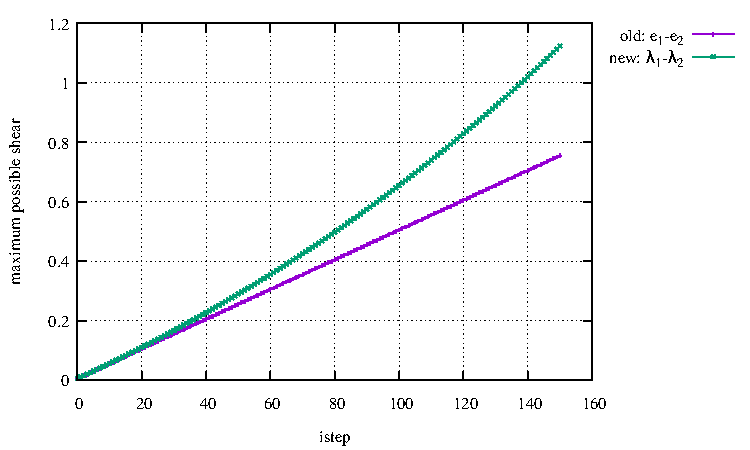
\includegraphics[width=5.5cm]{python_codes/fieldstone_89/results/vertical/maximum_shear.pdf}\\
{\captionfont Time evolution of the principal angle $\theta_\varepsilon$, 
the strain principal values and the area of the target cell.}
\end{center}





\newpage
%%%%%%%%%%%%%%%%%%%%%%%%%%%%%%%%%%%%%%%%%%%%%%%%%%%%%%%%%%%%%%%%%%%%%%5
\subsection*{Pure shear (experiment=3)}

\begin{eqnarray}
u(x,y)&=&x \\
v(x,y)&=&y
\end{eqnarray}


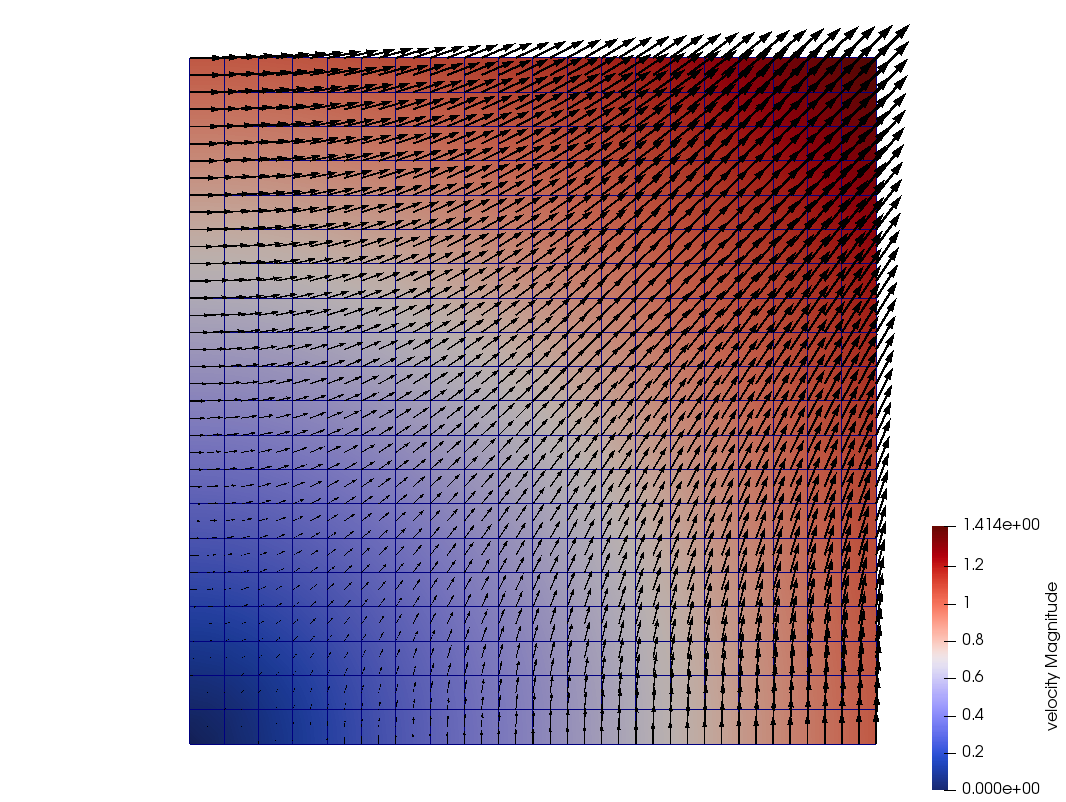
\includegraphics[width=5cm]{python_codes/fieldstone_89/results/pureshear/vel}


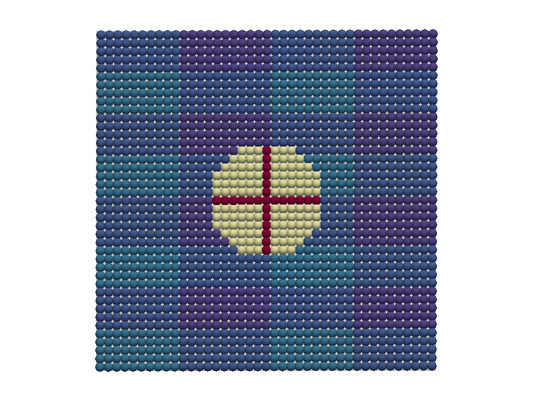
\includegraphics[width=5cm]{python_codes/fieldstone_89/results/pureshear/paint0000}
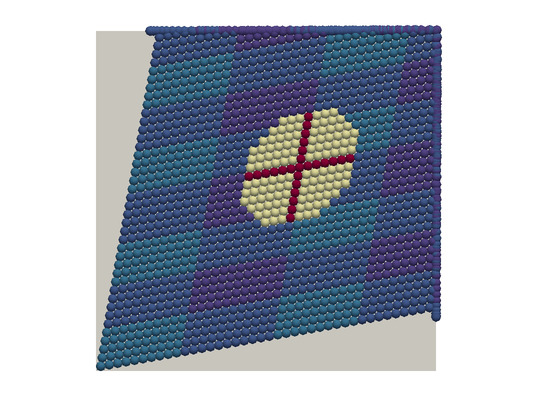
\includegraphics[width=5cm]{python_codes/fieldstone_89/results/pureshear/paint0005}
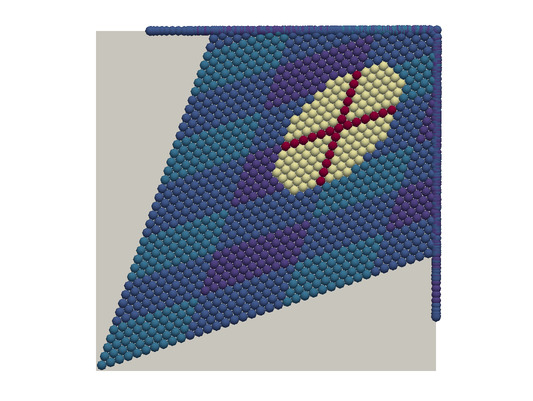
\includegraphics[width=5cm]{python_codes/fieldstone_89/results/pureshear/paint0010}

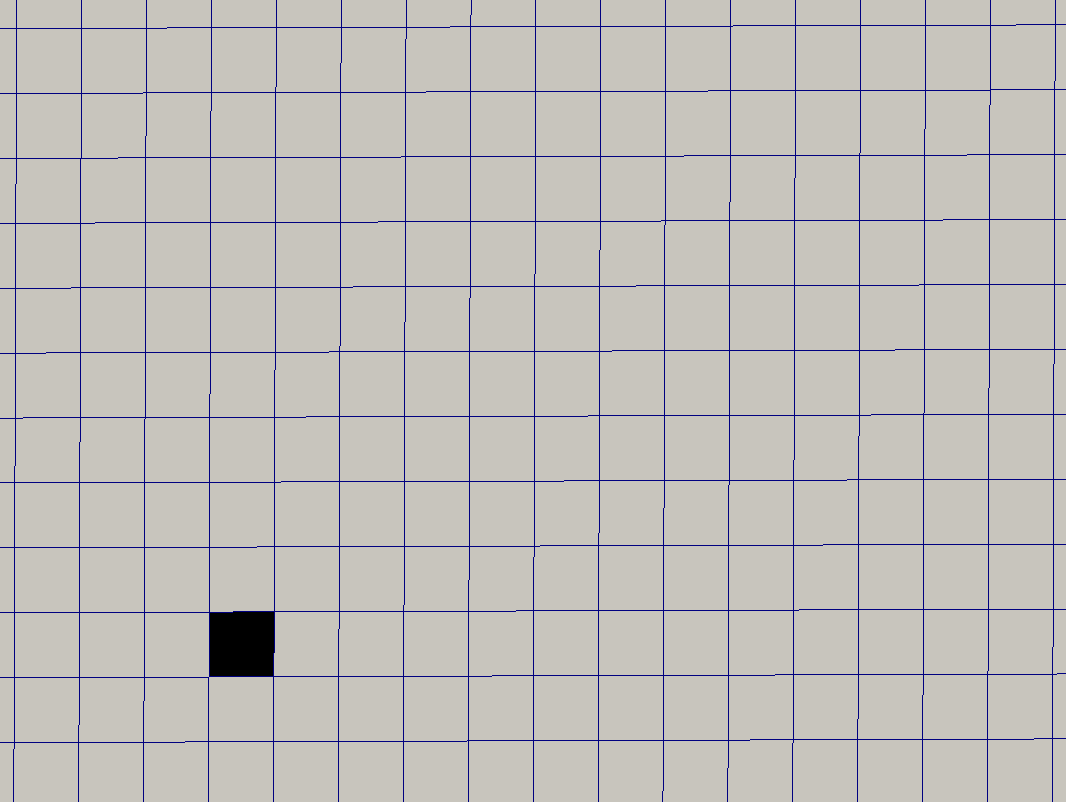
\includegraphics[width=5cm]{python_codes/fieldstone_89/results/pureshear/target0000}
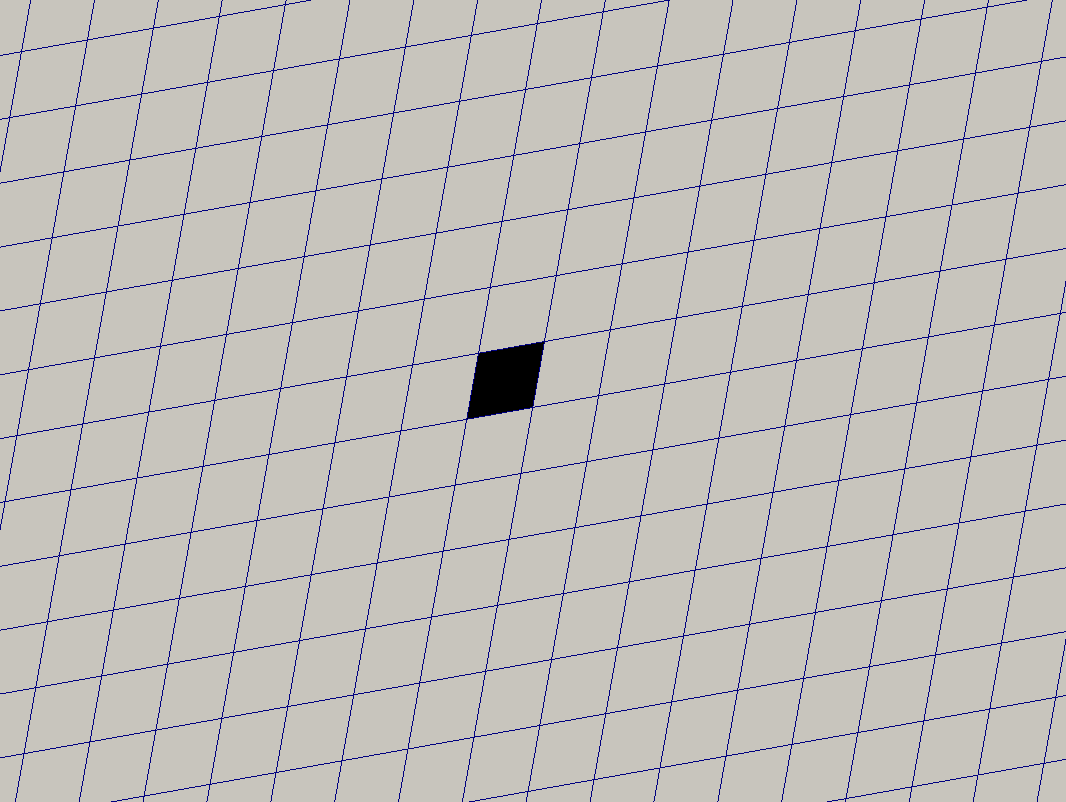
\includegraphics[width=5cm]{python_codes/fieldstone_89/results/pureshear/target0005}
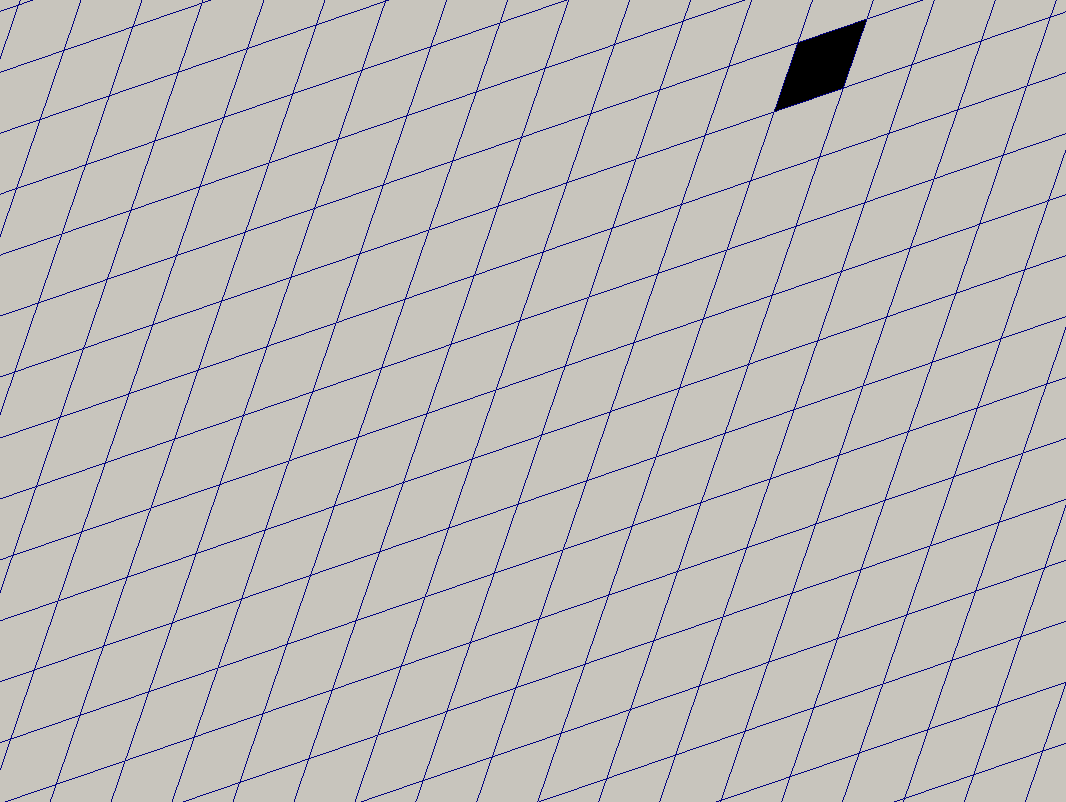
\includegraphics[width=5cm]{python_codes/fieldstone_89/results/pureshear/target0010}

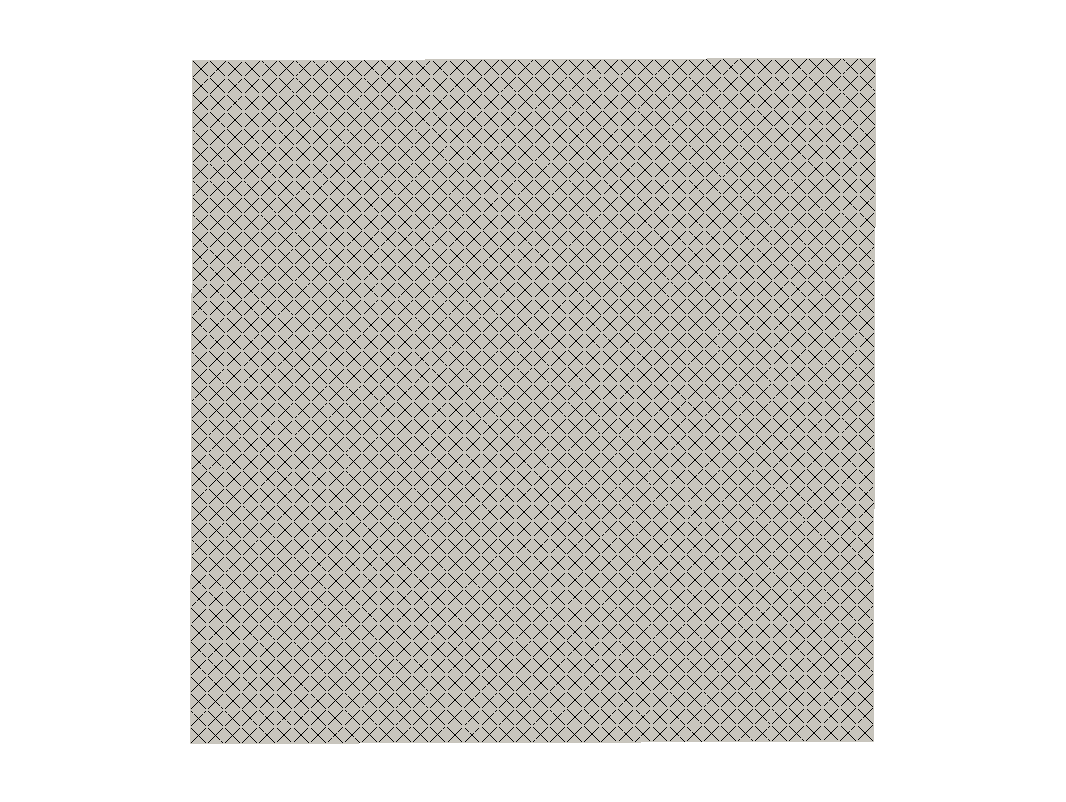
\includegraphics[width=5cm]{python_codes/fieldstone_89/results/pureshear/old_dirs0000}
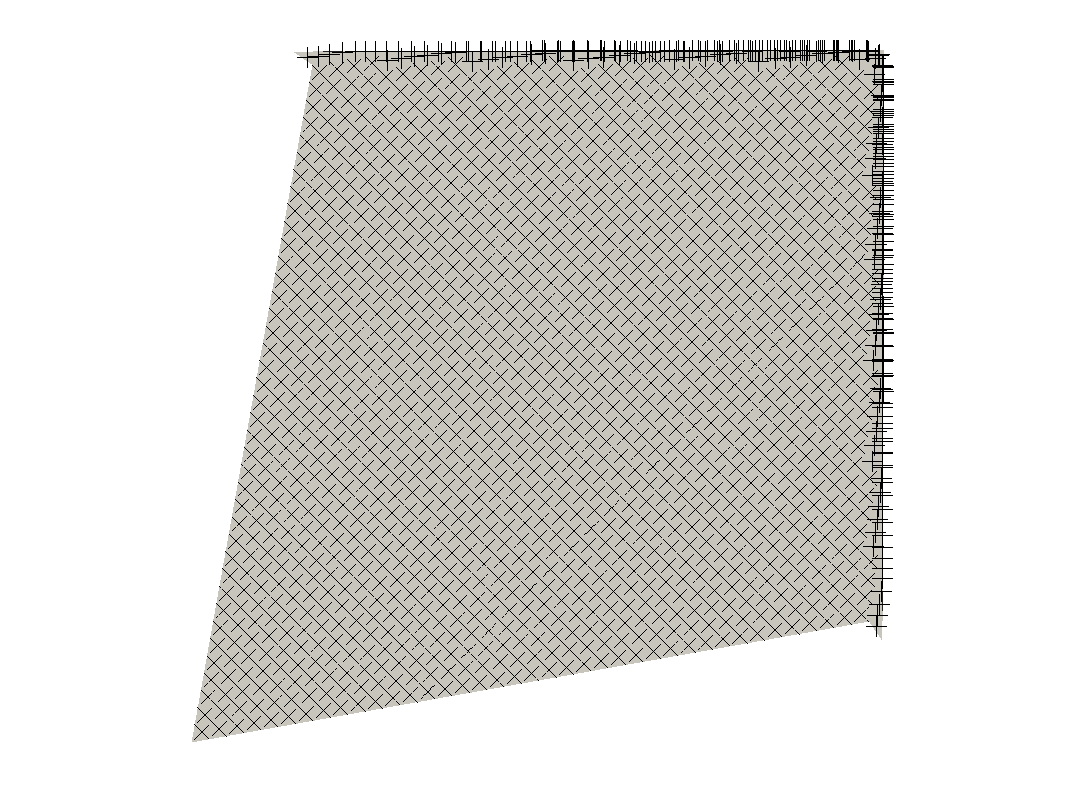
\includegraphics[width=5cm]{python_codes/fieldstone_89/results/pureshear/old_dirs0005}
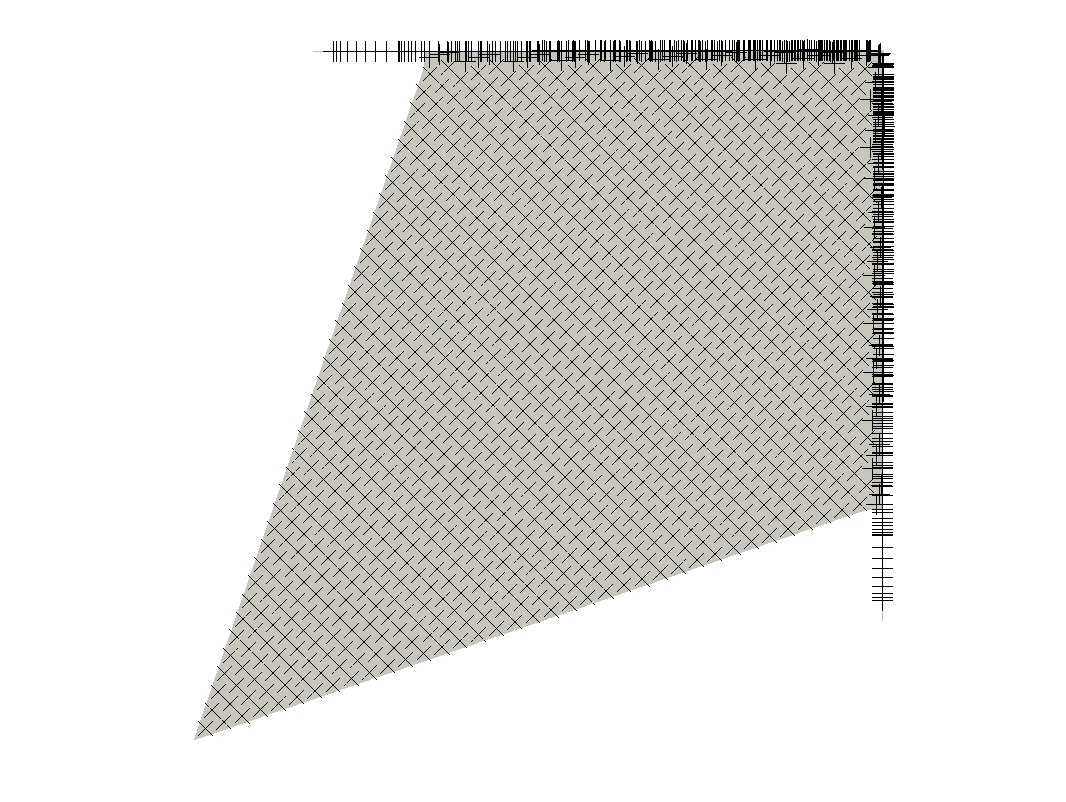
\includegraphics[width=5cm]{python_codes/fieldstone_89/results/pureshear/old_dirs0010}
{\captionfont old and new are identical}

\begin{center}
\includegraphics[width=5.5cm]{python_codes/fieldstone_89/results/pureshear/principal_angle.pdf}
\includegraphics[width=5.5cm]{python_codes/fieldstone_89/results/pureshear/principal_strains.pdf}
\includegraphics[width=5.5cm]{python_codes/fieldstone_89/results/pureshear/area.pdf}\\
\includegraphics[width=5.5cm]{python_codes/fieldstone_89/results/pureshear/R.pdf}
\includegraphics[width=5.5cm]{python_codes/fieldstone_89/results/pureshear/V.pdf}
\includegraphics[width=5.5cm]{python_codes/fieldstone_89/results/pureshear/maximum_shear.pdf}\\
{\captionfont Time evolution of the principal angle $\theta_\varepsilon$, 
the strain principal values and the area of the target cell.}
\end{center}

\newpage
%%%%%%%%%%%%%%%%%%%%%%%%%%%%%%%%%%%%%%%%%%%%%%%%%%%%%%%%%%%%%%%%%%%%%%5
\subsection*{Bi-axial extension (experiment=4)}

\begin{eqnarray}
u(x,y)&=&-x+L_x/2 \\
v(x,y)&=&y-L_y/2
\end{eqnarray}


\begin{center}
\includegraphics[width=5cm]{python_codes/fieldstone_89/results/biaxial/vel}
\end{center}


\begin{center}
\includegraphics[width=5cm]{python_codes/fieldstone_89/results/biaxial/target0000}
\includegraphics[width=5cm]{python_codes/fieldstone_89/results/biaxial/target0005}
\includegraphics[width=5cm]{python_codes/fieldstone_89/results/biaxial/target0010}
\end{center}

\begin{center}
\includegraphics[width=4cm]{python_codes/fieldstone_89/results/biaxial/paint0000}
\includegraphics[width=4cm]{python_codes/fieldstone_89/results/biaxial/paint0005}
\includegraphics[width=4cm]{python_codes/fieldstone_89/results/biaxial/paint0010}
\includegraphics[width=4cm]{python_codes/fieldstone_89/results/biaxial/paint0015}
\end{center}

\begin{center}
\includegraphics[width=4cm]{python_codes/fieldstone_89/results/biaxial/new_dirs0000}
\includegraphics[width=4cm]{python_codes/fieldstone_89/results/biaxial/new_dirs0005}
\includegraphics[width=4cm]{python_codes/fieldstone_89/results/biaxial/new_dirs0010}
\includegraphics[width=4cm]{python_codes/fieldstone_89/results/biaxial/new_dirs0015}
\end{center}

\begin{center}
\includegraphics[width=5.5cm]{python_codes/fieldstone_89/results/biaxial/principal_angle.pdf}
\includegraphics[width=5.5cm]{python_codes/fieldstone_89/results/biaxial/principal_strains.pdf}
\includegraphics[width=5.5cm]{python_codes/fieldstone_89/results/biaxial/area.pdf}\\
\includegraphics[width=5.5cm]{python_codes/fieldstone_89/results/biaxial/R.pdf}
\includegraphics[width=5.5cm]{python_codes/fieldstone_89/results/biaxial/V.pdf}
\includegraphics[width=5.5cm]{python_codes/fieldstone_89/results/biaxial/maximum_shear.pdf}\\
{\captionfont Time evolution of the principal angle $\theta_\varepsilon$, 
the strain principal values and the area of the target cell.}
\end{center}












\newpage
Message:

What I/the community does wrong:
on markers, we interpolate grav v through Q1 fcts , we compute $\dot{eps}_ij$, we
update the starin as $eps_ij += dot{eps}_ij$ . dt 
this is 'ok' only for (very) small total strains 
compare eigenvalues / principal strains $eps_1, eps_2$  


Malvern, then Taco have a better method to compute this total strain. 
We tesselate the marker swarm in quadrilaterals and we will compute
strain-related quantities in their centroids.

for each cell centroid, we compute the displacement gradient tensor F, 
then carry out polar decomposition to write F as product of stretch and rotation. 
F = R U  or F=  V R (we use the latter).
From V we compute the principal stretches (eigenvectors/values of V) bc
these represent the axes of the strain ellipse, i.e. directions of max stretch.
substract 1 to principal stretches to get principal strains, $eps_1,2 = lamda_1,2 - 1,2 $
compare these : the Malvern methid is supposefdly exact, so the difference tells me 
how bad my method is (up to few tens of \%) 
Also principal strains can never be smaller than -1 by def, because less than -1 means
more than 100\%  shortening (in 1D). but no upper limit.
conversely principal stretch > 0 (bc it is strain +1 ).







